\chapter{非光滑与复合优化}
\label{chap:opt-nonsmooth}

在最小二乘目标上加一项$\ell_1$正则，得到
\[
 \min_{\bm x\in\mathbb R^d}\ \frac12\lVert\bm A\bm x-\bm b\rVert_2^2+\lambda\lVert\bm x\rVert_1,
\]
人们希望它的解有许多坐标恰好为零。可是$\lvert x_j\rvert$恰好在$x_j=0$处有尖点，没有导数；第~\ref{chap:opt-smooth}章的梯度下降在这些点上无从计算更新；若随手取某一侧的斜率代替导数，坐标又容易在零的两侧来回跳动，很难恰好停在零上。最大值目标$\max_i\{\bm a_i^\top\bm x+b_i\}$也有同样的麻烦：哪一个分支最大发生切换的地方，函数图像形成一道折痕。机器学习中的稀疏正则、绝对值损失、合页损失和最坏情形目标，都会把这样的尖点带进优化问题。

于是要回答几件事。尖点处没有唯一的斜率，还剩下什么斜率信息，能否用它判断一个点已经最优？如果每次只能读到其中一条斜率，怎样累计进展，又该报告哪一个点？目标中非光滑的那一项往往很简单，例如$\ell_1$范数或某个凸集的指示函数，能不能完整保留它、只近似其余部分？当这一项既不简单、也不便单独处理时，能否换成一个有可控偏差的光滑函数，或者在迭代中逐轮建立更容易求解的模型？本章的学习目标，是为这些情形分别建立可计算的更新，并说清每种更新依赖什么条件、保证什么误差、返回哪一个点、每轮付出什么代价。

路线由“原目标能提供什么信息”决定。先在尖点处用全域支撑直线代替切线，得到次梯度与次微分，它们给出凸目标的最优条件；只读一条支撑斜率的次梯度法由此而来，它的保证落在历史最佳点或平均点上，而不是逐轮下降。若非光滑项本身可以连同一个二次距离项一起精确最小化，就得到邻近映射；闭凸集上的投影是它的特例。把邻近映射与第~\ref{chap:opt-smooth}章的二次上界结合，得到复合目标的邻近梯度法及其加速版本。最后两节处理没有便宜邻近映射的情形：光滑化用一个偏差已知的光滑函数整体替换原目标，代理模型则在每轮重新构造上界或下界模型，并用原目标检验改善。约束的完整处理留给第~\ref{chap:constrained-optimization}章，抽样带来的误差留给第~\ref{chap:opt-stochastic-block}章。

\section{非光滑目标与最优条件}
\label{sec:opt-ns-optimality}

光滑目标的最优条件是梯度为零；它依赖每一点都有一条切线。本节先看尖点处还能保留哪些斜率信息：对凸目标，保留的是所有全域有效的支撑直线，由此得到次梯度、次微分以及“零属于次微分”的全局最优判据。随后计算常见目标的次微分，并整理求和与复合规则。最后作为补充说明，失去凸性后只能退回局部斜率集合，它给出的只是必要条件。

本节沿用第~\ref{chap:optimization}章的扩展实值写法：目标$f:\mathbb R^d\to\mathbb R\cup\{+\infty\}$，有效定义域$\operatorname{dom}f=\{\bm x:f(\bm x)<+\infty\}$；$f$称为适当的，是指它不取$-\infty$且$\operatorname{dom}f$非空。约束$\bm x\in C$可以写成加上指示函数$\iota_C$，它在$C$上取$0$、在$C$外取$+\infty$。

\subsection{凸次梯度与次微分}
\label{sec:opt-ns-subgradient-def}

先看最简单的尖点$f(x)=|x|$。在$x=0$右侧，函数沿斜率$1$上升；在左侧，沿斜率$-1$上升。一条直线无法同时匹配两侧，所以经典导数不存在。但第~\ref{chap:optimization}章已经说明，可微凸函数的切线总在图像下方：
\[
 f(\bm y)\geq f(\bm x)+\langle\nabla f(\bm x),\bm y-\bm x\rangle\quad\text{对所有}\ \bm y.
\]
在$|x|$的原点，切线不存在，“处处在图像下方并在当前点接触”的直线却有一整族：$y=gx$只要$-1\leq g\leq1$就满足$|y|\geq gy$。图~\ref{fig:opt-ns-abs-supports}(a)画出了其中几条。把这种全域支撑作为新的斜率信息，就得到下面的定义。

\begin{definition}[次梯度与次微分]
\label{def:opt-ns-subgradient}
设$f:\mathbb R^d\to\mathbb R\cup\{+\infty\}$是适当凸函数，$\bm x\in\operatorname{dom}f$。若向量$\bm g\in\mathbb R^d$满足
\begin{equation}
 f(\bm y)\geq f(\bm x)+\langle\bm g,\bm y-\bm x\rangle\quad\text{对所有}\ \bm y\in\mathbb R^d,
 \label{eq:opt-ns-subgradient-inequality}
\end{equation}
就称$\bm g$为$f$在$\bm x$处的\term{次梯度}（subgradient）。$f$在$\bm x$处全部次梯度组成的集合称为\term{次微分}（subdifferential），记为$\partial f(\bm x)$；对$\bm x\notin\operatorname{dom}f$，约定$\partial f(\bm x)=\varnothing$。
\end{definition}

不等式~\eqref{eq:opt-ns-subgradient-inequality}要求仿射函数$\bm y\mapsto f(\bm x)+\langle\bm g,\bm y-\bm x\rangle$在整个空间位于$f$的下方，并在$\bm x$处与$f$相等。这是一个全域条件，不是只在$\bm x$附近成立的局部近似。对每个固定的$\bm y$，满足该不等式的$\bm g$构成一个闭半空间；$\partial f(\bm x)$是所有这些闭半空间的交，因此总是闭凸集，但它可能是空集，也可能含不止一个向量。

\begin{example}[绝对值的次微分]
\label{ex:opt-ns-abs-subdifferential}
对$f(x)=|x|$逐点计算。在$x=0$处，条件是$|y|\geq gy$对所有$y$成立；取$y=1$得$g\leq1$，取$y=-1$得$g\geq-1$，反过来$|g|\leq1$时$gy\leq|g||y|\leq|y|$，所以$\partial f(0)=[-1,1]$。在$x>0$处，取$y=x+s$，$|s|<x$，条件化为$x+s\geq x+gs$，即$s\geq gs$：$s>0$时得$g\leq1$，$s<0$时得$g\geq1$，所以只能$g=1$；而$g=1$确实满足$|y|\geq y$。同理$x<0$时$\partial f(x)=\{-1\}$。
\end{example}

图~\ref{fig:opt-ns-abs-supports}(b)把这个结果画成集合值映射：离开原点时，次微分是导数构成的单点；到了原点，它变成一整段竖直线段。读者应从图中看到，尖点并没有“丢失”斜率信息，而是同时保留了左右两侧之间的全部斜率。由此也要避免一种误读：$[-1,1]$中任取一个数都只是一条支撑斜率，不能称为原点处“唯一的导数”。

\begin{figure}[!htbp]
  \centering
  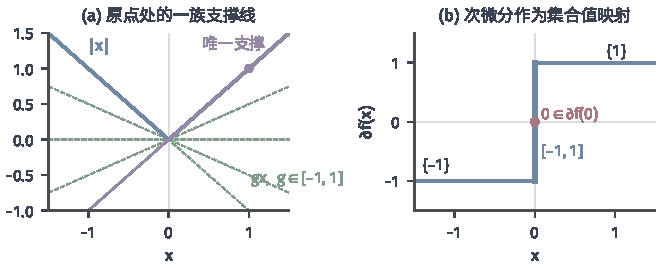
\includegraphics[width=112mm]{figures/03-optimization-evolution-and-signals/01-optimization/matplotlib/c4-abs-supports/figure.pdf}
  \caption{绝对值函数的支撑线与次微分。(a) 蓝线是$|x|$；绿色虚线是斜率$g=-1,-0.5,0,0.5,1$的直线$y=gx$，它们都在$|x|$下方并在原点接触。紫线是$x=1$处唯一的支撑线$y=x$，它与该点的切线重合。(b) 次微分$\partial|x|$：负半轴为$\{-1\}$，正半轴为$\{1\}$，原点处为竖直线段$[-1,1]$，其中含$0$（红点）。}
  \label{fig:opt-ns-abs-supports}
\end{figure}

\paragraph{可微点处的次微分}
在可微点，次微分应当回到梯度。设$f$凸，$\bm x$是$\operatorname{dom}f$的内点且$f$在$\bm x$可微。一方面，第~\ref{chap:optimization}章的一阶支撑不等式说明$\nabla f(\bm x)\in\partial f(\bm x)$。另一方面，若$\bm g\in\partial f(\bm x)$，对任意方向$\bm v$和小的$t>0$，取$\bm y=\bm x+t\bm v$得$f(\bm x+t\bm v)-f(\bm x)\geq t\langle\bm g,\bm v\rangle$；两边除以$t$并令$t\downarrow0$，得$\langle\nabla f(\bm x),\bm v\rangle\geq\langle\bm g,\bm v\rangle$。取$\bm v=\bm g-\nabla f(\bm x)$，即得$-\lVert\bm g-\nabla f(\bm x)\rVert_2^2\geq0$，所以$\bm g=\nabla f(\bm x)$。因此$\partial f(\bm x)=\{\nabla f(\bm x)\}$：次微分只在不可微处才可能多于一个元素。

\paragraph{零次梯度与全局最优}
支撑不等式最直接的用途是判定最优。若$\bm 0\in\partial f(\bm x^\star)$，把$\bm g=\bm 0$代入式~\eqref{eq:opt-ns-subgradient-inequality}就得到$f(\bm y)\geq f(\bm x^\star)$对所有$\bm y$成立；反过来，若$\bm x^\star\in\operatorname{dom}f$是全局最小点，则$f(\bm y)\geq f(\bm x^\star)+\langle\bm 0,\bm y-\bm x^\star\rangle$，即$\bm 0\in\partial f(\bm x^\star)$。

\begin{theorem}[凸目标的最优条件]
\label{thm:opt-ns-zero-subgradient}
设$f:\mathbb R^d\to\mathbb R\cup\{+\infty\}$是适当凸函数，$\bm x^\star\in\operatorname{dom}f$。则$\bm x^\star$是$f$在$\mathbb R^d$上的全局最小点，当且仅当$\bm 0\in\partial f(\bm x^\star)$。
\end{theorem}

这个判据要求的是“集合中含零”，而不是“次微分只有零”，更不是“算法这一轮取到的次梯度为零”。在$|x|$的原点，次微分是$[-1,1]$，它含零，所以原点最优；一个只返回一条支撑斜率的程序可能在原点报告$g=0.7$，这个非零读数并不否定最优性。反过来，只要某一轮确实读到了零次梯度，当前点就已被证明是全局最小点。

\paragraph{次微分可能为空}
定义域边界上可能没有任何支撑直线。取$f(x)=-\sqrt x$（$x\geq0$），在$x<0$时令$f(x)=+\infty$；它是适当凸函数。在$x=0$处，若$g$是次梯度，则对所有$y>0$有$-\sqrt y\geq gy$，即$g\leq-1/\sqrt y$；令$y\downarrow0$，右端趋于$-\infty$，不存在这样的$g$，所以$\partial f(0)=\varnothing$。图像在原点处是竖直切线，任何非竖直直线都会在原点右侧穿到图像上方。这个点不是最小点，与定理~\ref{thm:opt-ns-zero-subgradient}并不矛盾；它提醒我们，依赖“查询一条次梯度”的算法必须先确认查询点处确实能取得次梯度。在$\operatorname{dom}f$的内点处，适当凸函数的次微分总是非空的有界集，这是凸分析中的标准结论\sidecite[第23节]{rockafellar1970convex}；本章的次梯度算法例都只在这样的点上查询，例如目标在全空间取有限值的情形。

\subsection{次微分的计算}
\label{sec:opt-ns-subdifferential-calculus}

有了定义，下一步是把常见目标的次微分算出来。计算时要分清两件事：给出某一条支撑往往很容易，算法也常常只需要一条；而写出全部次微分，则需要说明没有遗漏的支撑。最优性判断用到的是后者。

\paragraph{范数与可分目标}
欧氏范数$f(\bm x)=\lVert\bm x\rVert_2$在$\bm x\neq\bm 0$处可微，梯度为$\bm x/\lVert\bm x\rVert_2$，所以$\partial f(\bm x)=\{\bm x/\lVert\bm x\rVert_2\}$。在原点，条件是$\lVert\bm y\rVert_2\geq\langle\bm g,\bm y\rangle$对所有$\bm y$成立：若$\lVert\bm g\rVert_2\leq1$，Cauchy--Schwarz不等式给出该条件；若$\lVert\bm g\rVert_2>1$，取$\bm y=\bm g$得$\lVert\bm g\rVert_2\geq\lVert\bm g\rVert_2^2$，矛盾。因此$\partial\lVert\cdot\rVert_2(\bm 0)$是闭单位球$\{\bm g:\lVert\bm g\rVert_2\leq1\}$，绝对值例中的区间$[-1,1]$是它在一维的情形。

若目标逐坐标分离，$f(\bm x)=\sum_{j=1}^df_j(x_j)$，其中每个$f_j$是一元适当凸函数，则
\begin{equation}
 \partial f(\bm x)=\partial f_1(x_1)\times\cdots\times\partial f_d(x_d).
 \label{eq:opt-ns-separable-subdifferential}
\end{equation}
右边包含于左边：把各坐标的支撑不等式相加即得。左边包含于右边：设$\bm g\in\partial f(\bm x)$，只改变第$j$个坐标、令其余坐标保持$x_i$，支撑不等式化为$f_j(y_j)\geq f_j(x_j)+g_j(y_j-x_j)$，即$g_j\in\partial f_j(x_j)$。对$\ell_1$范数$\lVert\bm x\rVert_1=\sum_j|x_j|$，这给出：$x_j\neq0$的坐标上$g_j=\operatorname{sign}(x_j)$，$x_j=0$的坐标上$g_j$可取$[-1,1]$中任意值。例如$\partial\lVert\cdot\rVert_1(2,0,-3)=\{1\}\times[-1,1]\times\{-1\}$。

\paragraph{有限仿射最大值}
设$f(\bm x)=\max_{1\leq i\leq m}\{\bm a_i^\top\bm x+b_i\}$，记在$\bm x$处取到最大值的指标集合为$I(\bm x)$，称这些分支为活跃分支。每个活跃分支都是一条支撑：对$i\in I(\bm x)$，有
\[
 f(\bm y)\geq\bm a_i^\top\bm y+b_i=f(\bm x)+\bm a_i^\top(\bm y-\bm x).
\]
次微分是凸集，所以活跃斜率的任何凸组合也是次梯度。反过来，次微分中没有别的向量。

\begin{theorem}[最大值函数的次微分]
\label{thm:opt-ns-max-subdifferential}
对$f(\bm x)=\max_{1\leq i\leq m}\{\bm a_i^\top\bm x+b_i\}$，有
\[
 \partial f(\bm x)=\operatorname{conv}\{\bm a_i:i\in I(\bm x)\},
\]
其中$\operatorname{conv}$表示\term{凸包}（convex hull），即有限个点全部凸组合构成的集合。
\end{theorem}

\begin{proof}
包含关系“$\supseteq$”已在定理前说明。为证“$\subseteq$”，设$\bm g\in\partial f(\bm x)$，记$P=\operatorname{conv}\{\bm a_i:i\in I(\bm x)\}$。$P$是有限个点的凸包，是非空紧凸集，所以连续函数$\bm a\mapsto\lVert\bm g-\bm a\rVert_2^2$在$P$上取得最小值，设最小点为$\bm p$。对任意$\bm a\in P$和$s\in(0,1]$，$\bm p+s(\bm a-\bm p)\in P$，由最小性
\[
 \lVert\bm g-\bm p\rVert_2^2\leq\lVert\bm g-\bm p-s(\bm a-\bm p)\rVert_2^2
 =\lVert\bm g-\bm p\rVert_2^2-2s\langle\bm g-\bm p,\bm a-\bm p\rangle+s^2\lVert\bm a-\bm p\rVert_2^2;
\]
消去相同项、除以$s$并令$s\downarrow0$，得$\langle\bm g-\bm p,\bm a-\bm p\rangle\leq0$。

若$\bm g\notin P$，令$\bm v=\bm g-\bm p\neq\bm 0$，则对每个$\bm a\in P$，
\[
 \langle\bm g,\bm v\rangle-\langle\bm a,\bm v\rangle
 =\langle\bm g-\bm p,\bm v\rangle+\langle\bm p-\bm a,\bm g-\bm p\rangle
 \geq\lVert\bm v\rVert_2^2>0.
\]
另一方面，非活跃分支在$\bm x$处严格小于$f(\bm x)$，由连续性，对足够小的$t>0$它们在$\bm x+t\bm v$处仍不活跃，于是
\[
 f(\bm x+t\bm v)=\max_{i\in I(\bm x)}\{\bm a_i^\top\bm x+b_i+t\bm a_i^\top\bm v\}=f(\bm x)+t\max_{i\in I(\bm x)}\bm a_i^\top\bm v.
\]
支撑不等式给出$f(\bm x+t\bm v)\geq f(\bm x)+t\langle\bm g,\bm v\rangle$，从而$\max_{i\in I(\bm x)}\bm a_i^\top\bm v\geq\langle\bm g,\bm v\rangle$，与上式矛盾。故$\bm g\in P$。
\end{proof}

证明中“紧凸集上最近点满足的内积不等式”在第~\ref{sec:opt-ns-prox-computation}小节还会对一般闭凸集系统地建立；这里只用到有限点凸包这一紧的情形。

\begin{example}[一维三段折线]
\label{ex:opt-ns-three-pieces}
取$f(x)=\max\{-x,\ x/2,\ 2x-3\}$。三条直线两两求交可知：$x\leq0$时$-x$最大，$0\leq x\leq2$时$x/2$最大，$x\geq2$时$2x-3$最大。于是在$x=0$处活跃分支为$-x$与$x/2$，$\partial f(0)=\operatorname{conv}\{-1,1/2\}=[-1,1/2]$；在$x=2$处$\partial f(2)=[1/2,2]$；其余点次微分是单个斜率。因为$0\in[-1,1/2]$，由定理~\ref{thm:opt-ns-zero-subgradient}，$x^\star=0$是全局最小点，$f^\star=0$。图~\ref{fig:opt-ns-max-affine}左图在两个切换点各画出几条支撑线，右图是$\partial f$的图像：每到一个切换点，次微分就从左侧斜率跳到右侧斜率，并在切换点处填满两者之间的整段。
\end{example}

\begin{figure}[!htbp]
  \centering
  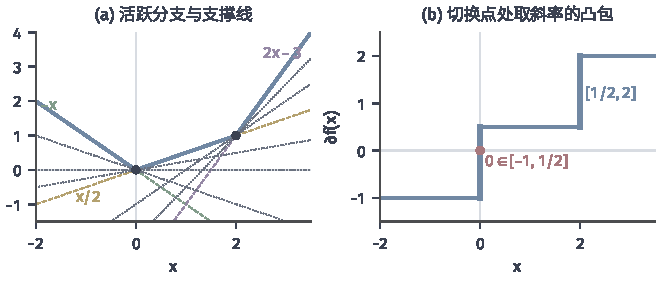
\includegraphics[width=112mm]{figures/03-optimization-evolution-and-signals/01-optimization/matplotlib/c4-max-affine-subdiff/figure.pdf}
  \caption{有限仿射最大值$f(x)=\max\{-x,x/2,2x-3\}$的次微分。(a) 蓝线是$f$，三条彩色虚线是各分支的延长线；灰色点线是切换点$x=0$与$x=2$处的几条支撑线，斜率分别取自$[-1,1/2]$与$[1/2,2]$。(b) $\partial f(x)$的图像：在切换点处取活跃斜率的凸包（竖直线段），红点标出$0\in\partial f(0)$。}
  \label{fig:opt-ns-max-affine}
\end{figure}

\paragraph{运算规则}
计算更复杂的目标，需要把次微分与加法、数乘和线性变换联系起来。对正数$\alpha>0$，支撑不等式两边同乘$\alpha$即得$\partial(\alpha f)(\bm x)=\alpha\,\partial f(\bm x)$。对仿射复合$h(\bm x)=f(\bm B\bm x+\bm c)$，若$\bm u\in\partial f(\bm B\bm x+\bm c)$，则
\[
 h(\bm y)\geq h(\bm x)+\langle\bm u,\bm B(\bm y-\bm x)\rangle=h(\bm x)+\langle\bm B^\top\bm u,\bm y-\bm x\rangle,
\]
所以$\bm B^\top\partial f(\bm B\bm x+\bm c)\subseteq\partial h(\bm x)$。同理，把两个支撑不等式相加，总有
\begin{equation}
 \partial f_1(\bm x)+\partial f_2(\bm x)\subseteq\partial(f_1+f_2)(\bm x).
 \label{eq:opt-ns-sum-inclusion}
\end{equation}

这两个包含关系的反方向都可能失败，而反方向恰恰是最优性判断需要的：若只知道$\bm 0\in\partial(f_1+f_2)(\bm x)$，却无法把它拆成两项次梯度之和，就不能写出逐项的最优条件。下面的例子说明失败确实会发生。在$\mathbb R$上取$f_1(x)=-\sqrt x$（$x\geq0$，否则为$+\infty$），$f_2=\iota_{(-\infty,0]}$。和函数只在$x=0$处有限，它就是单点集$\{0\}$的指示函数，$\partial(f_1+f_2)(0)=\mathbb R$；但前面已算出$\partial f_1(0)=\varnothing$，所以左边是空集，等式不成立。问题出在两个有效定义域只在一个边界点接触。

为了表述“定义域充分重叠”，需要相对内部的概念。$\mathbb R^d$中凸集$S$的\term{相对内部}（relative interior）$\operatorname{ri}S$，是把$S$放在它的仿射包（包含$S$的最小仿射集）中考察时的内部。例如平面中一条线段没有普通意义的内点，它的相对内部是去掉两个端点的开线段；全空间的相对内部就是全空间。

\begin{theorem}[次微分的求和与复合规则]
\label{thm:opt-ns-sum-rule}
设$f_1,f_2:\mathbb R^d\to\mathbb R\cup\{+\infty\}$是适当凸函数。若$\operatorname{ri}(\operatorname{dom}f_1)\cap\operatorname{ri}(\operatorname{dom}f_2)\neq\varnothing$，则对所有$\bm x$，
\[
 \partial(f_1+f_2)(\bm x)=\partial f_1(\bm x)+\partial f_2(\bm x).
\]
类似地，若$f$是适当凸函数且存在$\bm x_0$使$\bm B\bm x_0+\bm c\in\operatorname{ri}(\operatorname{dom}f)$，则$\partial h(\bm x)=\bm B^\top\partial f(\bm B\bm x+\bm c)$。
\end{theorem}

这两个等式的证明需要凸集分离定理，可参考前面引用的凸分析教材第23节，本章不展开。最常用的情形是其中一项在全空间取有限值：此时它的定义域是$\mathbb R^d$，相对内部条件自动成立。例如Lasso目标$\frac12\lVert\bm A\bm x-\bm b\rVert_2^2+\lambda\lVert\bm x\rVert_1$的两项都处处有限，于是
\[
 \partial\Bigl(\frac12\lVert\bm A\bm x-\bm b\rVert_2^2+\lambda\lVert\bm x\rVert_1\Bigr)
 =\bm A^\top(\bm A\bm x-\bm b)+\lambda\,\partial\lVert\bm x\rVert_1,
\]
最优条件是：$x_j\neq0$的坐标上$[\bm A^\top(\bm b-\bm A\bm x)]_j=\lambda\operatorname{sign}(x_j)$，$x_j=0$的坐标上$|[\bm A^\top(\bm b-\bm A\bm x)]_j|\leq\lambda$。一维情形$\min_x\frac12(x-3)^2+|x|$中，$x=2$满足$0\in(2-3)+\{1\}$，所以$x^\star=2$。

只有包含关系~\eqref{eq:opt-ns-sum-inclusion}时，仍然可以从“拆出的两项之和含零”推出最优，但不能反过来要求每个最小点都能这样拆分。第~\ref{sec:opt-ns-prox}节的邻近最优条件将直接用函数值比较推出，不依赖求和等式。

\subsection{非凸广义驻点（补充）}
\label{sec:opt-ns-clarke}

本小节说明失去凸性以后，尖点处的斜率信息会退化成什么；后面各节的主要结论都在凸情形下给出，跳过本小节不影响阅读。

对非凸函数，全域支撑常常不存在。$f(x)=-|x|$在原点没有任何次梯度：若$g$是次梯度，取$y=1$得$-1\geq g$，取$y=-1$得$-1\geq-g$，二者不能同时成立。可是原点处仍有清楚的局部斜率信息：两侧的导数分别是$1$和$-1$。为了保留这种信息，改为收集附近可微点上梯度的极限。

\paragraph{Clarke广义梯度}
称$f$在开集$U\subseteq\mathbb R^d$上局部Lipschitz，是指每一点都有一个邻域，在其中$|f(\bm y)-f(\bm z)|\leq K\lVert\bm y-\bm z\rVert_2$对某个常数$K$成立。这类函数在$U$中几乎处处可微，这是Rademacher定理的结论；它保证了下面的极限有足够多的可微点可取。对$\bm x\in U$，令
\[
 \partial^\circ f(\bm x)=\operatorname{conv}\Bigl\{\lim_{k\to\infty}\nabla f(\bm x_k):\bm x_k\to\bm x,\ f\text{ 在 }\bm x_k\text{ 可微，且极限存在}\Bigr\},
\]
称为\term{Clarke广义梯度}（Clarke generalized gradient）\sidecite{math-clarke1990optimization}。局部Lipschitz保证这些梯度有界，因而这是非空紧凸集。

对$|x|$与$-|x|$，原点两侧的梯度分别是$\pm1$，所以两者在原点的Clarke广义梯度都是$[-1,1]$。图~\ref{fig:opt-ns-clarke}把两种情形并排画出：两幅图中$g=0$的水平线都与这个集合相容，左图中它是全域支撑，右图中原函数却处处在它下方。同一个斜率集合，可以对应局部最小点，也可以对应局部最大点。对局部Lipschitz的凸函数，Clarke广义梯度与凸次微分一致（见前引专著第2.2节），所以它确实是次微分的推广。

\begin{figure}[!htbp]
  \centering
  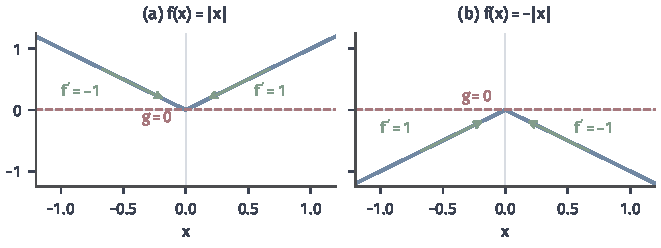
\includegraphics[width=112mm]{figures/03-optimization-evolution-and-signals/01-optimization/matplotlib/c4-clarke-abs/figure.pdf}
  \caption{同一个Clarke广义梯度对应不同的局部性质。蓝线分别是$|x|$与$-|x|$，绿色箭头标出原点两侧的导数，它们的凸包都是$[-1,1]$；红色虚线是斜率$g=0$的直线。(a) 中这条直线是全域支撑，原点是全局最小点；(b) 中原函数处处在它下方，原点是局部最大点，凸次微分为空集。}
  \label{fig:opt-ns-clarke}
\end{figure}

\paragraph{含零只是必要条件}
Clarke广义梯度有一个等价刻画：定义允许基点移动的方向导数
\[
 f^\circ(\bm x;\bm v)=\limsup_{\bm y\to\bm x,\ t\downarrow0}\frac{f(\bm y+t\bm v)-f(\bm y)}{t},
\]
则$\partial^\circ f(\bm x)=\{\bm g:\langle\bm g,\bm v\rangle\leq f^\circ(\bm x;\bm v)\ \text{对所有}\ \bm v\}$（同一专著第2.1节与第2.5节）。若$\bm x$是局部最小点，在上极限中固定$\bm y=\bm x$，对足够小的$t>0$分子$f(\bm x+t\bm v)-f(\bm x)\geq0$，所以$f^\circ(\bm x;\bm v)\geq0$对所有$\bm v$成立；由等价刻画，$\bm 0\in\partial^\circ f(\bm x)$。这说明局部极小点一定是\term{Clarke驻点}（Clarke stationary point）。

反方向不成立：$-|x|$的原点满足$0\in\partial^\circ f(0)$，却是局部最大点。凸情形中“含零”之所以能推出全局最优，靠的是全域支撑不等式；Clarke广义梯度只记录局部斜率，没有这样的不等式。因此对非凸目标，算法找到Clarke驻点只是满足了一个必要条件；要接回全局最优判据，需要额外证明目标凸，或在问题结构中找到别的证书。

\paragraph{弱凸性}
介于凸与一般非凸之间，有一类负曲率受控的函数。若存在$\rho\geq0$使$f+\frac\rho2\lVert\cdot\rVert_2^2$是凸函数，称$f$为\term{$\rho$弱凸}（$\rho$-weakly convex）。例如$\cos x$的二阶导数不小于$-1$，所以$\cos x+x^2/2$凸，$\cos x$是$1$弱凸的；$|x^2-1|$在$|x|<1$上的二阶导数为$-2$、在两个尖点处是凸的折角，所以它是$2$弱凸的。$-|x|$则不是任何$\rho$下的弱凸函数：加上光滑二次项改变不了原点处向下的折角。

对$\rho$弱凸函数，凸函数$f+\frac\rho2\lVert\cdot\rVert_2^2$的支撑不等式改写后成为
\[
 f(\bm y)\geq f(\bm x)+\langle\bm g,\bm y-\bm x\rangle-\frac\rho2\lVert\bm y-\bm x\rVert_2^2,
\]
其中$\bm g\in\partial\bigl(f+\frac\rho2\lVert\cdot\rVert_2^2\bigr)(\bm x)-\rho\bm x$：全域仿射下界换成了向下开口的二次下界。这一下界让第~\ref{sec:opt-ns-prox}节的邻近子问题在适当参数下保持可解。但弱凸并不保证驻点是全局最优：$|x^2-1|$在$x=0$处可微、导数为零，却是局部最大点。它也不是强凸性或第~\ref{chap:opt-smooth}章中梯度控制目标差的那类条件的同义词：弱凸只限制最坏的负曲率，不提供任何正曲率。

\section{次梯度方法}
\label{sec:opt-ns-subgradient-methods}

上一节说明了尖点处保留的是一整组支撑斜率。实际的计算程序通常拿不到整组斜率：给定查询点，它返回函数值和其中一条次梯度。本节研究只凭这样的信息怎样推进。最直接的做法是把梯度下降中的梯度换成次梯度；我们会看到，这一替换保留了“靠近最小点”的性质，却失去了“目标逐轮下降”的性质，所以必须重新规定算法返回哪一个点、报告什么误差。

\subsection{更新与返回对象}
\label{sec:opt-ns-subgradient-update}

设$f:\mathbb R^d\to\mathbb R$是凸函数（在全空间取有限值，因而每一点都有次梯度），计算程序对任意查询点$\bm x$返回$f(\bm x)$和某个$\bm g\in\partial f(\bm x)$。我们不能假定返回的是哪一条次梯度；分析必须对任意选择成立。\term{次梯度法}（subgradient method）的一轮更新是
\begin{equation}
 \bm x^{(t+1)}=\bm x^{(t)}-\eta^{(t)}\bm g^{(t)},\qquad\bm g^{(t)}\in\partial f(\bm x^{(t)}),
 \label{eq:opt-ns-subgradient-update}
\end{equation}
其中$\eta^{(t)}>0$是预先规定的步长。目标若取扩展实值，更新后的点可能落到$\operatorname{dom}f$之外，那里既没有有限函数值也没有次梯度；这时需要把更新点投影回可行集，相应的投影次梯度法在第~\ref{chap:constrained-optimization}章讨论。本节只处理全空间有限值的目标。

\paragraph{负次梯度未必是下降方向}
梯度下降之所以能用小步长保证下降，是因为$-\nabla f(\bm x)$与目标的局部变化相匹配：沿它走一小步$s$，一阶变化是$-s\lVert\nabla f(\bm x)\rVert_2^2<0$。次梯度不再有这种匹配。先看一维的例子：$f(x)=|x|$，从$x^{(0)}=0.2$以步长$1$沿$-\operatorname{sign}(x)$走，得到$x^{(1)}=-0.8$，目标从$0.2$升到$0.8$。这里的失败可以归咎于步长太大、跨过了尖点。

更本质的情况是，有些负次梯度方向对任何正步长都会使目标上升。取$f(\bm x)=|x_1|+2|x_2|$与$\bm x=(1,0)^\top$。由可分规则~\eqref{eq:opt-ns-separable-subdifferential}，$\partial f(\bm x)=\{1\}\times[-2,2]$，所以$\bm g=(1,2)^\top$是一条合法的次梯度。沿$-\bm g$走步长$s\in(0,1)$，
\[
 f(\bm x-s\bm g)=|1-s|+2|-2s|=1+3s>1=f(\bm x),
\]
无论$s$多小，目标都上升。同一点的另一条次梯度$(1,0)^\top$却是下降方向。图~\ref{fig:opt-ns-subgrad-not-descent}把这一现象画在等高线上：红色箭头$-\bm g$离开了$f=1$的菱形等高线，进入了目标更大的区域。

\begin{figure}[!htbp]
  \centering
  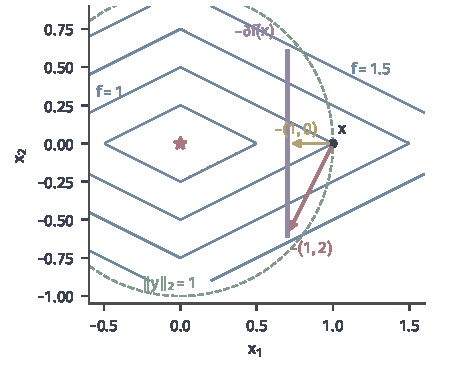
\includegraphics[width=80mm]{figures/03-optimization-evolution-and-signals/01-optimization/matplotlib/c4-subgrad-not-descent/figure.pdf}
  \caption{负次梯度方向可能使目标上升，却仍然靠近最小点。蓝色菱形是$f(\bm x)=|x_1|+2|x_2|$的等高线（$f=0.5,1,1.5,2$），红星是最小点$\bm 0$。在$\bm x=(1,0)^\top$处，次微分$\{1\}\times[-2,2]$的负向（按$0.3$倍缩放）画成紫色竖线段。红色箭头沿$-(1,2)^\top$，越出$f=1$的等高线，目标上升；黄色箭头沿$-(1,0)^\top$，目标下降。绿色虚线是以最小点为圆心、过$\bm x$的圆：两支箭头的终点都在圆内。}
  \label{fig:opt-ns-subgrad-not-descent}
\end{figure}

\paragraph{负次梯度靠近最小点}
图中还有一个容易忽略的事实：红色箭头虽然使目标上升，却进入了以最小点为圆心、过当前点的圆内。这不是巧合。设$\bm x^\star$是任一最小点，$\bm g\in\partial f(\bm x)$，把支撑不等式~\eqref{eq:opt-ns-subgradient-inequality}用于$\bm y=\bm x^\star$，得$\langle\bm g,\bm x-\bm x^\star\rangle\geq f(\bm x)-f^\star$。于是
\begin{equation}
 \begin{aligned}
 \lVert\bm x-s\bm g-\bm x^\star\rVert_2^2
 &=\lVert\bm x-\bm x^\star\rVert_2^2-2s\langle\bm g,\bm x-\bm x^\star\rangle+s^2\lVert\bm g\rVert_2^2\\
 &\leq\lVert\bm x-\bm x^\star\rVert_2^2-2s\bigl(f(\bm x)-f^\star\bigr)+s^2\lVert\bm g\rVert_2^2.
 \end{aligned}
 \label{eq:opt-ns-distance-one-step}
\end{equation}
其中$s>0$是步长。只要$\bm x$不是最小点、$s$足够小，右端就严格小于$\lVert\bm x-\bm x^\star\rVert_2^2$。在上面的例子中，$\lVert\bm x-s\bm g\rVert_2^2=(1-s)^2+4s^2=1-2s+5s^2$，$0<s<2/5$时小于$1$。次梯度方法的进展是用到最小点的距离来衡量的，而不是用目标值；这一点决定了下面的返回规则和下一小节的分析。

\paragraph{历史最佳点与加权平均点}
既然目标值可以在某一轮上升，最后一个迭代点就不一定是目前找到的最好点。算法因此要维护一个返回对象，常用的有两种：历史最佳点$\bm x_{\mathrm{best}}^{(T)}$，即$\bm x^{(0)},\dots,\bm x^{(T-1)}$中目标值最小的一个；以及按步长加权的平均点
\[
 \bar{\bm x}^{(T)}=\frac{\sum_{t=0}^{T-1}\eta^{(t)}\bm x^{(t)}}{\sum_{t=0}^{T-1}\eta^{(t)}}.
\]
最佳点需要每轮的函数值；平均点不需要函数值，但要额外维护一个加权和。

\begin{algorithm}[次梯度法]
  \label{alg:opt-ns-subgradient}
  \begin{algorithmic}[1]
    \Require 在全空间有限的凸函数$f$的函数值与次梯度程序；初值$\bm x^{(0)}$；步长$\eta^{(0)},\dots,\eta^{(T-1)}>0$；预算$T$
    \Ensure 历史最佳点$\bm x_{\mathrm{best}}$、加权平均点$\bar{\bm x}$及相应目标值
    \State $f_{\mathrm{best}}\gets+\infty$，$\bm s\gets\bm 0$，$W\gets0$
    \For{$t=0,1,\dots,T-1$}
      \State 查询$f(\bm x^{(t)})$与一个$\bm g^{(t)}\in\partial f(\bm x^{(t)})$
      \If{$f(\bm x^{(t)})<f_{\mathrm{best}}$}
        \State $f_{\mathrm{best}}\gets f(\bm x^{(t)})$，$\bm x_{\mathrm{best}}\gets\bm x^{(t)}$
      \EndIf
      \If{$\bm g^{(t)}=\bm 0$}
        \State \Return $\bm x^{(t)}$（零次梯度已证明它是全局最小点）
      \EndIf
      \State $\bm s\gets\bm s+\eta^{(t)}\bm x^{(t)}$，$W\gets W+\eta^{(t)}$
      \State $\bm x^{(t+1)}\gets\bm x^{(t)}-\eta^{(t)}\bm g^{(t)}$
    \EndFor
    \State $\bar{\bm x}\gets\bm s/W$，计算$f(\bar{\bm x})$
    \State \Return $\bm x_{\mathrm{best}}$、$\bar{\bm x}$及其目标值
  \end{algorithmic}
\end{algorithm}

算法~\ref{alg:opt-ns-subgradient}每轮的代价是一次函数值与次梯度查询，加上$O(d)$的向量运算。注意更新顺序：当前点先参与最佳点和平均点的记录，然后才被替换；下一小节的误差界针对的正是这些被查询过的点。

\paragraph{停止时能报告什么}
光滑情形常用梯度范数作停止准则，次梯度范数却不能直接替代它。在$|x|$的原点，程序可能返回$g=1$，范数为$1$，而原点已是最优。真正与最优性对应的量是零到整个次微分的距离$\operatorname{dist}(\bm 0,\partial f(\bm x))=\min\{\lVert\bm g\rVert_2:\bm g\in\partial f(\bm x)\}$：由定理~\ref{thm:opt-ns-zero-subgradient}，它为零当且仅当$\bm x$最优。若它等于$\delta$，又已知$\lVert\bm x-\bm x^\star\rVert_2\leq R$，取达到最小范数的$\bm g$代入支撑不等式，得
\[
 f(\bm x)-f^\star\leq\langle\bm g,\bm x-\bm x^\star\rangle\leq\delta R.
\]
可惜计算这个距离需要整个次微分，而查询程序只给一条次梯度。

因此，次梯度法通常按预算停止，并报告返回点、其目标值和所依据的假设。若另有一个可信的下界$\ell\leq f^\star$（例如来自第~\ref{chap:constrained-optimization}章的对偶问题，或问题本身已知最小值非负），就可以报告可核验的目标间隙$f(\bm x_{\mathrm{best}})-\ell$，它是$f(\bm x_{\mathrm{best}})-f^\star$的上界。没有下界时，只能报告下一小节在相应假设下给出的理论界。

\subsection{步长与有限步误差}
\label{sec:opt-ns-subgradient-rate}

不等式~\eqref{eq:opt-ns-distance-one-step}说明每一步都在用目标差换取距离的减小，同时付出一项与步长平方成正比的代价。把这种交换沿迭代累加，就得到次梯度法的有限步误差界。

\begin{theorem}[次梯度法的有限步误差]
\label{thm:opt-ns-subgradient-rate}
设$f:\mathbb R^d\to\mathbb R$凸，最小点$\bm x^\star$存在，$\lVert\bm x^{(0)}-\bm x^\star\rVert_2\leq R$，并且算法实际取到的次梯度满足$\lVert\bm g^{(t)}\rVert_2\leq G$（$t=0,\dots,T-1$）。则
\begin{equation}
 \min_{0\leq t<T}f(\bm x^{(t)})-f^\star\leq\frac{R^2+G^2\sum_{t=0}^{T-1}(\eta^{(t)})^2}{2\sum_{t=0}^{T-1}\eta^{(t)}},
 \label{eq:opt-ns-subgradient-bound}
\end{equation}
并且加权平均点$\bar{\bm x}^{(T)}$满足同样的界。
\end{theorem}

\begin{proof}
对每一轮应用式~\eqref{eq:opt-ns-distance-one-step}（取$\bm x=\bm x^{(t)}$、$s=\eta^{(t)}$、$\bm g=\bm g^{(t)}$），整理得
\[
 2\eta^{(t)}\bigl(f(\bm x^{(t)})-f^\star\bigr)\leq\lVert\bm x^{(t)}-\bm x^\star\rVert_2^2-\lVert\bm x^{(t+1)}-\bm x^\star\rVert_2^2+(\eta^{(t)})^2G^2.
\]
对$t=0,\dots,T-1$求和，右端距离项逐项相消，只剩$\lVert\bm x^{(0)}-\bm x^\star\rVert_2^2-\lVert\bm x^{(T)}-\bm x^\star\rVert_2^2\leq R^2$，所以
\[
 2\sum_{t=0}^{T-1}\eta^{(t)}\bigl(f(\bm x^{(t)})-f^\star\bigr)\leq R^2+G^2\sum_{t=0}^{T-1}(\eta^{(t)})^2.
\]
左端每一项都不小于$2\eta^{(t)}\bigl(\min_sf(\bm x^{(s)})-f^\star\bigr)$，除以$2\sum_t\eta^{(t)}$即得式~\eqref{eq:opt-ns-subgradient-bound}。对平均点，凸性给出$f(\bar{\bm x}^{(T)})\leq\sum_t\eta^{(t)}f(\bm x^{(t)})/\sum_t\eta^{(t)}$，左端的加权平均同样被上式控制。
\end{proof}

这个界只对历史最佳点和平均点成立，没有说最后一个迭代点$\bm x^{(T)}$怎样。它的分子由两部分组成：$R^2$是初始距离的代价，要靠累计步长$\sum_t\eta^{(t)}$去摊薄；$G^2\sum_t(\eta^{(t)})^2$是每步越过尖点的代价，随步长平方累积。步长的选择就是平衡这两项。

\paragraph{已知预算的固定步长}
若预先知道要做$T$步，取常数步长$\eta$，右端变为$\dfrac{R^2}{2T\eta}+\dfrac{G^2\eta}{2}$。两项一个随$\eta$减小、一个随$\eta$增大，在$\eta=R/(G\sqrt T)$处相等，此时
\[
 \min_{0\leq t<T}f(\bm x^{(t)})-f^\star\leq\frac{RG}{\sqrt T}.
\]
要把目标差压到$\varepsilon$，需要约$(RG/\varepsilon)^2$次查询。若不按预算调整、始终使用某个固定$\eta$，$T\to\infty$时界停在$G^2\eta/2$，不会趋于零。

\begin{example}[固定步长的平台]
\label{ex:opt-ns-subgradient-plateau}
对$f(x)=|x|$取$x^{(0)}=1$、$\eta=0.3$，取$g^{(t)}=\operatorname{sign}(x^{(t)})$。迭代依次为$1,\ 0.7,\ 0.4,\ 0.1,\ -0.2,\ 0.1,\ -0.2,\dots$：第三步以后在$0.1$与$-0.2$之间来回，历史最佳目标值停在$0.1$。这里$R=G=1$，定理给出的界$(1+0.09T)/(0.6T)$随$T$增大趋于$0.15$，与实际的$0.1$一致地停在一个正的平台上。步长不缩小，尖点处的来回跳动就不会停止。
\end{example}

\paragraph{预算未知的递减步长}
若事先不知道要做多少步，取$\eta^{(t)}=R/(G\sqrt{t+1})$。由于$T$个加数$1/\sqrt{t+1}$都不小于$1/\sqrt T$，累计步长$\sum_{t<T}\eta^{(t)}\geq(R/G)\sqrt T$；而$\sum_{t<T}1/(t+1)\leq1+\ln T$，所以平方和$\sum_{t<T}(\eta^{(t)})^2\leq(R/G)^2(1+\ln T)$。代入式~\eqref{eq:opt-ns-subgradient-bound}，
\[
 \min_{0\leq t<T}f(\bm x^{(t)})-f^\star\leq\frac{RG(2+\ln T)}{2\sqrt T},
\]
比已知预算的情形多一个对数因子。更一般地，只要$\sum_t\eta^{(t)}=\infty$而$\sum_t(\eta^{(t)})^2/\sum_t\eta^{(t)}\to0$，右端就趋于零。

图~\ref{fig:opt-ns-subgrad-steps}在$f(\bm x)=|x_1|+2|x_2|$上比较三种步长，初值$(1.47,0.93)^\top$，次梯度取$(\operatorname{sign}x_1,2\operatorname{sign}x_2)^\top$（约定$\operatorname{sign}0=0$），于是$R\approx1.74$、$G=\sqrt5$。左图是$\eta=0.1$的路径：迭代很快到达$x_2=0$附近，此后在横轴两侧锯齿形前进，到达最小点附近后不再收缩。右图的曲线显示，$\eta=0.1$在十几步内就到达平台，却停在约$0.17$；$\eta=0.01$起步慢，平台低到约$0.02$；递减步长没有平台，2000步时约为$0.013$，并始终位于灰色参考线$RG/\sqrt T$附近或其下方。

\begin{figure}[!htbp]
  \centering
  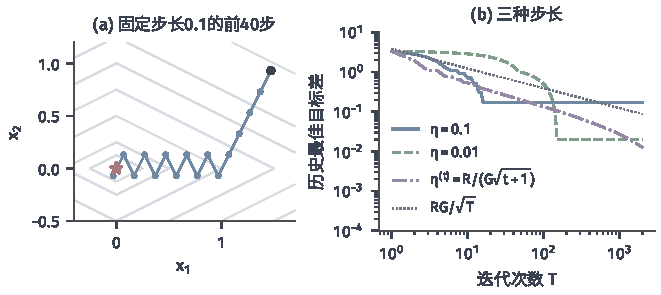
\includegraphics[width=112mm]{figures/03-optimization-evolution-and-signals/01-optimization/matplotlib/c4-subgrad-steps/figure.pdf}
  \caption{次梯度法的步长与锯齿。目标$f(\bm x)=|x_1|+2|x_2|$，最小点为原点（红星），初值$(1.47,0.93)^\top$。(a) 固定步长$\eta=0.1$的前40步：到达横轴附近后在两侧来回跳动。(b) 历史最佳目标差随迭代次数的变化（双对数坐标）：固定步长$0.1$与$0.01$分别停在约$0.17$与$0.02$的平台，递减步长$\eta^{(t)}=R/(G\sqrt{t+1})$持续下降；灰色点线为参考量$RG/\sqrt T$。}
  \label{fig:opt-ns-subgrad-steps}
\end{figure}

\paragraph{几种量不能互相替代}
次梯度法的分析中出现了几个容易混淆的量。累计步长$\sum_t\eta^{(t)}$是摊薄初始距离所需的“时间”；实际路径长度$\sum_t\eta^{(t)}\lVert\bm g^{(t)}\rVert_2$还含次梯度范数，在锯齿阶段会持续增长；目标误差是定理~\ref{thm:opt-ns-subgradient-rate}控制的对象；参数$\bm x^{(t)}$是否收敛到某个最小点，又是另一回事。上面的定理只给出返回点的目标误差，没有断言迭代序列收敛，也没有断言路径长度有限。在锯齿例中，路径长度随步数线性增长，目标误差却停在平台：二者都不能代替对方说明算法的状态。

\section{邻近映射与隐式更新}
\label{sec:opt-ns-prox}

次梯度法每轮只取一条支撑斜率，尖点处其余的形状信息全部丢掉了，这正是它在尖点附近来回跳动的原因。若非光滑函数足够简单，可以换一种做法：不读取它的斜率，而是把它完整地放进一个小的优化子问题，再加一项“不要离当前点太远”的二次惩罚。本节先建立这种子问题的解，即邻近映射，证明它存在唯一、刻画它的最优条件和稳定性；然后计算几类常用函数的邻近映射，其中闭凸集上的投影是一个特例；最后把整个目标放进邻近子问题，得到邻近点法。下一节的复合方法会把这一运算与光滑部分的梯度步组合起来。

\subsection{邻近映射的定义与性质}
\label{sec:opt-ns-prox-def}

给定中心$\bm z$和函数$r$，考虑子问题
\[
 \min_{\bm x}\ r(\bm x)+\frac1{2\eta}\lVert\bm x-\bm z\rVert_2^2 .
\]
只最小化$r$，解可能离$\bm z$很远，甚至不存在；只最小化距离项，解就是$\bm z$本身，$r$没有得到任何改善。二者相加，参数$\eta>0$决定两者的相对分量：$\eta$小时距离项占主导，解贴近$\bm z$；$\eta$大时$r$的作用增强。

图~\ref{fig:opt-ns-prox-subproblem}在$r(w)=|w|$、$\eta=1$下画出两个中心对应的子问题。可以把它想成一根连在$z$上的弹簧拉着点$w$，弹簧的拉力是$(z-w)/\eta$；而$|w|$像一块有摩擦的地面，在$w\neq0$时始终以大小为$1$的力把$w$推向原点，在$w=0$处则能提供$[-1,1]$中任意大小的阻力。$z=0.5$时，弹簧在原点的拉力只有$0.5$，摩擦挡得住，解停在$0$；$z=2$时，弹簧把点拉到$w=1$，此时拉力$1$恰好与摩擦力平衡。这个类比对应的正是下面的最优条件$(\bm z-\bm p)/\eta\in\partial r(\bm p)$：拉力必须是$r$在解处的某条次梯度。

\begin{figure}[!htbp]
  \centering
  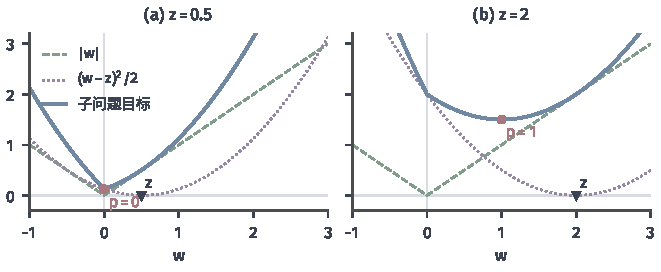
\includegraphics[width=112mm]{figures/03-optimization-evolution-and-signals/01-optimization/matplotlib/c4-prox-subproblem/figure.pdf}
  \caption{邻近子问题$|w|+(w-z)^2/2$（$\eta=1$）。绿色虚线是非光滑项$|w|$，紫色点线是以中心$z$（黑色三角）为最低点的二次距离项，蓝线是两者之和，红点是子问题的最小点$p$。(a) $z=0.5$时$p=0$：在原点处$z-p=0.5$落在$\partial|\cdot|(0)=[-1,1]$中。(b) $z=2$时$p=1$：$z-p=1$恰等于$|\cdot|$在$1$处的斜率。}
  \label{fig:opt-ns-prox-subproblem}
\end{figure}

要让这个子问题对任何中心都有唯一的解，需要对$r$提出条件。回顾第~\ref{chap:optimization}章：$r$下半连续，是指$\bm x_k\to\bm x$时总有$r(\bm x)\leq\liminf_kr(\bm x_k)$；下半连续函数若有非空的紧下水平集，就能取得最小值。

\begin{definition}[邻近映射]
\label{def:opt-ns-prox}
设$r:\mathbb R^d\to\mathbb R\cup\{+\infty\}$是适当、下半连续的凸函数，$\eta>0$。对每个$\bm z\in\mathbb R^d$，令
\begin{equation}
 \operatorname{prox}_{\eta r}(\bm z)=\argmin_{\bm x\in\mathbb R^d}\Bigl\{r(\bm x)+\frac1{2\eta}\lVert\bm x-\bm z\rVert_2^2\Bigr\},
 \label{eq:opt-ns-prox-def}
\end{equation}
称$\operatorname{prox}_{\eta r}$为$r$（以参数$\eta$）的\term{邻近映射}（proximal mapping），也称\term{邻近算子}（proximal operator）。
\end{definition}

定义中把$\argmin$写成一个点，需要先证明最小点存在且唯一。下面的定理同时给出它的最优条件；证明只用函数值比较，不依赖次微分的求和等式。

\begin{theorem}[邻近映射的存在唯一与最优条件]
\label{thm:opt-ns-prox-characterization}
在定义~\ref{def:opt-ns-prox}的条件下，对每个$\bm z$，子问题~\eqref{eq:opt-ns-prox-def}有唯一最小点$\bm p$。并且对$\bm p\in\operatorname{dom}r$，以下三条等价：
\begin{enumerate}
  \item $\bm p=\operatorname{prox}_{\eta r}(\bm z)$；
  \item $(\bm z-\bm p)/\eta\in\partial r(\bm p)$；
  \item 对所有$\bm y$，$r(\bm y)+\dfrac1{2\eta}\lVert\bm y-\bm z\rVert_2^2\geq r(\bm p)+\dfrac1{2\eta}\lVert\bm p-\bm z\rVert_2^2+\dfrac1{2\eta}\lVert\bm y-\bm p\rVert_2^2$。
\end{enumerate}
\end{theorem}

\begin{proof}
\emph{存在。}记子问题目标为$\phi(\bm x)=r(\bm x)+\lVert\bm x-\bm z\rVert_2^2/(2\eta)$。先说明$r$至多以线性速度向$-\infty$下降。取$\bm x_0\in\operatorname{dom}r$。$r$下半连续，在紧集$\{\bm x:\lVert\bm x-\bm x_0\rVert_2\leq1\}$上取得最小值$m$，$m$有限且$m\leq r(\bm x_0)$。对$\lVert\bm x-\bm x_0\rVert_2>1$，令$\theta=1/\lVert\bm x-\bm x_0\rVert_2$，点$\bm u=(1-\theta)\bm x_0+\theta\bm x$在这个单位球面上，凸性给出$m\leq r(\bm u)\leq(1-\theta)r(\bm x_0)+\theta r(\bm x)$，整理得
\[
 r(\bm x)\geq r(\bm x_0)-\bigl(r(\bm x_0)-m\bigr)\lVert\bm x-\bm x_0\rVert_2 .
\]
因此$\phi(\bm x)\geq r(\bm x_0)-c\lVert\bm x-\bm x_0\rVert_2+\lVert\bm x-\bm z\rVert_2^2/(2\eta)$，其中$c=r(\bm x_0)-m\geq0$。二次项最终压过线性项，$\phi$的每个下水平集都有界；$\phi$下半连续，所以下水平集是闭集，从而是紧集。$\phi(\bm x_0)<+\infty$保证下水平集$\{\phi\leq\phi(\bm x_0)\}$非空，由第~\ref{chap:optimization}章的存在性结论，最小点存在。

\emph{(1)$\Rightarrow$(2)。}设$\bm p$是最小点，任取$\bm y$与$\theta\in(0,1)$，令$\bm p_\theta=\bm p+\theta(\bm y-\bm p)$。由最小性和$r$的凸性，
\[
 \begin{aligned}
 r(\bm p)+\frac{\lVert\bm p-\bm z\rVert_2^2}{2\eta}
 &\leq r(\bm p_\theta)+\frac{\lVert\bm p_\theta-\bm z\rVert_2^2}{2\eta}\\
 &\leq(1-\theta)r(\bm p)+\theta r(\bm y)+\frac{\lVert\bm p-\bm z\rVert_2^2}{2\eta}\\
 &\qquad+\frac\theta\eta\langle\bm p-\bm z,\bm y-\bm p\rangle+\frac{\theta^2}{2\eta}\lVert\bm y-\bm p\rVert_2^2.
 \end{aligned}
\]
消去相同项、除以$\theta$，再令$\theta\downarrow0$，得$r(\bm y)\geq r(\bm p)+\langle(\bm z-\bm p)/\eta,\bm y-\bm p\rangle$，这正是(2)。

\emph{(2)$\Rightarrow$(3)。}由(2)，$r(\bm y)\geq r(\bm p)+\frac1\eta\langle\bm z-\bm p,\bm y-\bm p\rangle$。再利用恒等式
\[
 \lVert\bm y-\bm z\rVert_2^2=\lVert\bm y-\bm p\rVert_2^2+2\langle\bm y-\bm p,\bm p-\bm z\rangle+\lVert\bm p-\bm z\rVert_2^2,
\]
两式相加后内积项恰好抵消，即得(3)。

\emph{(3)$\Rightarrow$(1)与唯一性。}(3)说明$\phi(\bm y)\geq\phi(\bm p)+\lVert\bm y-\bm p\rVert_2^2/(2\eta)$，所以$\bm p$是最小点，并且任何$\bm y\neq\bm p$的目标值都严格更大，最小点唯一。
\end{proof}

条件(2)可以读成一个隐式的次梯度步：$\bm p=\bm z-\eta\bm g$，其中$\bm g\in\partial r(\bm p)$。与次梯度法的显式步$\bm z-\eta\bm g$、$\bm g\in\partial r(\bm z)$相比，斜率是在新点而不是旧点读取的。条件(3)比最小性更强：解的目标值比任何其他候选至少低一个二次量，后面分析邻近梯度法和邻近点法时都要用它。

\paragraph{子问题的解不是原问题的解}
$\operatorname{prox}_{\eta r}(\bm z)$是一个强凸子问题的解，一般不是$r$本身的最小点。在图~\ref{fig:opt-ns-prox-subproblem}(b)中，$|w|$的最小点是$0$，子问题的解却是$1$。两者重合的情形可以准确刻画：由条件(2)，$\operatorname{prox}_{\eta r}(\bm z)=\bm z$当且仅当$\bm 0\in\partial r(\bm z)$，即$\bm z$是$r$的最小点。邻近映射的不动点恰好是原函数的最小点；这就是后面用反复调用邻近映射去求最小点的依据。

\paragraph{非扩张性}
设$\bm p_1=\operatorname{prox}_{\eta r}(\bm z_1)$，$\bm p_2=\operatorname{prox}_{\eta r}(\bm z_2)$。把条件(2)的支撑不等式分别用于对方的点：
\[
 r(\bm p_2)\geq r(\bm p_1)+\tfrac1\eta\langle\bm z_1-\bm p_1,\bm p_2-\bm p_1\rangle,\qquad
 r(\bm p_1)\geq r(\bm p_2)+\tfrac1\eta\langle\bm z_2-\bm p_2,\bm p_1-\bm p_2\rangle.
\]
两式相加，$r$的值抵消，得$\langle(\bm z_1-\bm z_2)-(\bm p_1-\bm p_2),\bm p_1-\bm p_2\rangle\geq0$，即
\begin{equation}
 \lVert\bm p_1-\bm p_2\rVert_2^2\leq\langle\bm z_1-\bm z_2,\bm p_1-\bm p_2\rangle\leq\lVert\bm z_1-\bm z_2\rVert_2\lVert\bm p_1-\bm p_2\rVert_2 .
 \label{eq:opt-ns-prox-firm}
\end{equation}
所以$\lVert\operatorname{prox}_{\eta r}(\bm z_1)-\operatorname{prox}_{\eta r}(\bm z_2)\rVert_2\leq\lVert\bm z_1-\bm z_2\rVert_2$：邻近映射是\term{非扩张映射}（nonexpansive mapping），中心的误差不会在一次调用中被放大。在迭代算法里，中心往往由带误差的梯度算出，这一性质保证一次邻近调用不会额外放大这个误差。

\paragraph{可解不等于便宜}
定理~\ref{thm:opt-ns-prox-characterization}只说明解存在唯一，没有说明它好算。对一般的$r$，求邻近映射本身就是一个与原问题难度相当的优化问题。邻近方法真正有用，是在$r$有闭式或可快速计算的邻近映射时，下一小节给出几类这样的函数。

\paragraph{弱凸函数的邻近映射}
若$r$不凸但是$\rho$弱凸，并且$0<\eta<1/\rho$，子问题目标$r+\frac1{2\eta}\lVert\cdot-\bm z\rVert_2^2$等于凸函数$r+\frac\rho2\lVert\cdot\rVert_2^2$加上一个系数为$\frac1{2\eta}-\frac\rho2>0$的二次函数，仍然强凸，解存在唯一。但非扩张性不再成立。取$r(x)=-\rho x^2/2$，子问题$-\rho x^2/2+(x-z)^2/(2\eta)$的驻点满足$-\rho x+(x-z)/\eta=0$，解为$\operatorname{prox}_{\eta r}(z)=z/(1-\eta\rho)$，它把中心的差放大了$1/(1-\eta\rho)>1$倍。弱凸推广因此必须限制参数$\eta$，并单独分析误差传播。

\subsection{邻近映射的计算}
\label{sec:opt-ns-prox-computation}

邻近方法的效率取决于邻近映射能否快速计算。本小节先推导$\ell_1$范数的软阈值并与二次正则对照，再把闭凸集的指示函数代入定义，得到投影及其性质。

\paragraph{软阈值}
取$r(\bm x)=\lambda\lVert\bm x\rVert_1$，$\lambda\geq0$。子问题目标$\sum_j\bigl(\lambda|x_j|+(x_j-z_j)^2/(2\eta)\bigr)$逐坐标分离，各坐标可以分别最小化。对一个坐标，由定理~\ref{thm:opt-ns-prox-characterization}的条件(2)，$p$是解当且仅当$(z-p)/\eta\in\lambda\,\partial|\cdot|(p)$。分三种情况：若$p>0$，需$z-p=\eta\lambda$，即$p=z-\eta\lambda$，这要求$z>\eta\lambda$；若$p<0$，同理$p=z+\eta\lambda$，要求$z<-\eta\lambda$；若$p=0$，需$z/\eta\in[-\lambda,\lambda]$，即$|z|\leq\eta\lambda$。三种情况恰好覆盖全部$z$，合起来就是\term{软阈值}（soft thresholding）
\begin{equation}
 \bigl[\operatorname{prox}_{\eta\lambda\lVert\cdot\rVert_1}(\bm z)\bigr]_j=\operatorname{sign}(z_j)\max\{|z_j|-\eta\lambda,0\}.
 \label{eq:opt-ns-soft-threshold}
\end{equation}
例如$\bm z=(3,0.4,-2)^\top$、$\eta\lambda=1$时，输出为$(2,0,-1)^\top$：大的坐标向原点平移$1$，小于阈值的坐标被精确置零。

把它与二次正则对照。$r(\bm x)=\frac\lambda2\lVert\bm x\rVert_2^2$可微，条件(2)化为$\bm z-\bm p=\eta\lambda\bm p$，解为$\bm p=\bm z/(1+\eta\lambda)$；同一输入得$(1.5,0.2,-1)^\top$。二次正则按比例收缩，任何非零坐标都不会变成零；$\ell_1$正则的零区间来自原点处次微分是整段区间：只要中心的拉力不超过阈值，解就停在零。图~\ref{fig:opt-ns-prox-maps}把两种映射与下面的区间投影画在同一坐标系中。

\begin{figure}[!htbp]
  \centering
  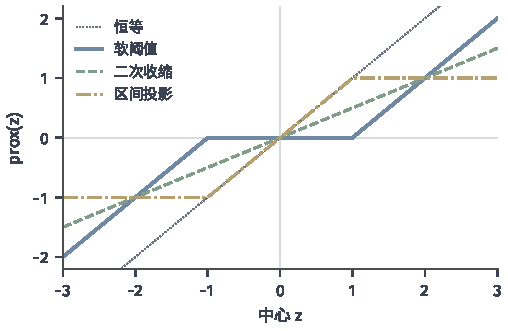
\includegraphics[width=86mm]{figures/03-optimization-evolution-and-signals/01-optimization/matplotlib/c4-prox-maps/figure.pdf}
  \caption{三种一维邻近映射（参数取$1$）。蓝线是$|w|$的软阈值$\operatorname{sign}(z)\max\{|z|-1,0\}$，在$[-1,1]$上恒为零；绿色虚线是$w^2/2$的二次收缩$z/2$，只在$z=0$处为零；黄色点划线是区间$[-1,1]$指示函数的邻近映射，即把$z$截断到区间内；灰色点线是恒等映射。三者都是非扩张的：曲线斜率不超过$1$。}
  \label{fig:opt-ns-prox-maps}
\end{figure}

\paragraph{加权与分组的阈值}
阈值来自原点处次微分的形状，换用别的范数时要重新核验。加权$\ell_1$范数$\sum_j\lambda_j|x_j|$仍然逐坐标分离，各坐标的阈值变为$\eta\lambda_j$。欧氏范数$r(\bm x)=\lambda\lVert\bm x\rVert_2$则不再分离：若$\bm p\neq\bm 0$，条件(2)要求$\bm z-\bm p=\eta\lambda\bm p/\lVert\bm p\rVert_2$，所以$\bm p$与$\bm z$同向，$\bm p=(1-\eta\lambda/\lVert\bm z\rVert_2)\bm z$，这要求$\lVert\bm z\rVert_2>\eta\lambda$；若$\bm p=\bm 0$，条件是$\bm z/\eta$属于$\lambda$倍单位球，即$\lVert\bm z\rVert_2\leq\eta\lambda$。于是
\[
 \operatorname{prox}_{\eta\lambda\lVert\cdot\rVert_2}(\bm z)=\max\Bigl\{1-\frac{\eta\lambda}{\lVert\bm z\rVert_2},0\Bigr\}\bm z ,
\]
整个向量要么一起置零、要么一起沿原方向缩短。对$\bm z=(3,4)^\top$、$\eta\lambda=1$，结果是$(2.4,3.2)^\top$；逐坐标软阈值却给出$(2,3)^\top$，两者不同。

\paragraph{投影}
约束$\bm x\in C$用指示函数$\iota_C$写入目标。设$C$是非空闭凸集，则$\iota_C$适当（$C$非空）、凸（$C$凸）、下半连续（$C$闭），满足定义~\ref{def:opt-ns-prox}的条件。代入定义，
\[
 \operatorname{prox}_{\eta\iota_C}(\bm z)=\argmin_{\bm x\in C}\frac1{2\eta}\lVert\bm x-\bm z\rVert_2^2=\argmin_{\bm x\in C}\lVert\bm x-\bm z\rVert_2 ,
\]
它与$\eta$无关，就是$C$中离$\bm z$最近的点，称为$\bm z$在$C$上的\term{投影}（projection），记为$\Pi_C(\bm z)$。定理~\ref{thm:opt-ns-prox-characterization}和非扩张性直接给出投影的基本性质。

\begin{theorem}[闭凸集上的投影]
\label{thm:opt-ns-projection}
设$C\subseteq\mathbb R^d$是非空闭凸集。则对每个$\bm z$，最近点$\bm p=\Pi_C(\bm z)$存在且唯一，并且$\bm p\in C$由下面的\term{变分不等式}（variational inequality）刻画：
\begin{equation}
 \langle\bm z-\bm p,\bm y-\bm p\rangle\leq0\quad\text{对所有}\ \bm y\in C.
 \label{eq:opt-ns-projection-vi}
\end{equation}
此外，对所有$\bm y\in C$有$\lVert\bm p-\bm y\rVert_2^2+\lVert\bm z-\bm p\rVert_2^2\leq\lVert\bm z-\bm y\rVert_2^2$，并且$\lVert\Pi_C(\bm z_1)-\Pi_C(\bm z_2)\rVert_2\leq\lVert\bm z_1-\bm z_2\rVert_2$。
\end{theorem}

\begin{proof}
存在唯一与非扩张性是定理~\ref{thm:opt-ns-prox-characterization}和式~\eqref{eq:opt-ns-prox-firm}在$r=\iota_C$时的特例。条件(2)写成$\iota_C(\bm y)\geq\iota_C(\bm p)+\frac1\eta\langle\bm z-\bm p,\bm y-\bm p\rangle$对所有$\bm y$成立；$\bm y\notin C$时左端为$+\infty$，自动成立，$\bm y\in C$时它就是式~\eqref{eq:opt-ns-projection-vi}。条件(3)取$\bm y\in C$、乘以$2\eta$，即得距离不等式。
\end{proof}

式~\eqref{eq:opt-ns-projection-vi}的几何意义是：从投影点$\bm p$指向原点$\bm z$的向量，与从$\bm p$指向$C$中任一点的向量夹角不小于直角。集合$\{\bm v:\langle\bm v,\bm y-\bm p\rangle\leq0\ \text{对所有}\ \bm y\in C\}$是一个闭凸锥，称为$C$在$\bm p$处的\term{法锥}（normal cone），记为$N_C(\bm p)$；它恰好就是$\partial\iota_C(\bm p)$。于是投影的最优条件可以说成：$\bm z-\Pi_C(\bm z)\in N_C(\Pi_C(\bm z))$，即“$\bm z$减去投影点后的残差必须沿法向”。在$C$的内点处法锥只有零向量，所以内点的投影只能是它自己；在光滑边界上法锥是一条外法线射线；在角点处法锥张成一个楔形区域。

\begin{example}[正方形上的投影]
\label{ex:opt-ns-box-projection}
取$C=[0,1]^2$。它的指示函数是两个区间指示函数之和，逐坐标分离，所以投影就是逐坐标截断：$[\Pi_C(\bm z)]_j=\min\{\max\{z_j,0\},1\}$。对$\bm z_a=(1.6,0.6)^\top$，投影$\bm p_a=(1,0.6)^\top$落在右边上，残差$(0.6,0)^\top$沿该边的外法线；对$C$中任一点$\bm y$，$\langle\bm z_a-\bm p_a,\bm y-\bm p_a\rangle=0.6(y_1-1)\leq0$。对$\bm z_b=(1.7,-0.5)^\top$，投影是顶点$\bm p_b=(1,0)^\top$，残差$(0.7,-0.5)^\top$；该顶点的法锥是$\{\bm v:v_1\geq0,\ v_2\leq0\}$，残差确实在其中。图~\ref{fig:opt-ns-projection}画出了这两种情形。
\end{example}

\begin{figure}[!htbp]
  \centering
  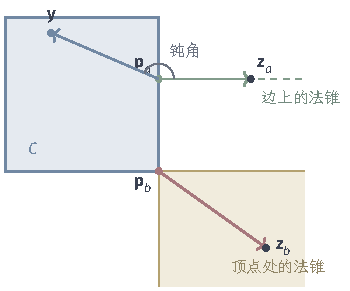
\includegraphics[width=59.33mm]{figures/03-optimization-evolution-and-signals/01-optimization/tikz/c4-projection-normal-cone/figure.pdf}
  \caption{正方形$C=[0,1]^2$上的投影与法锥。$\bm z_a=(1.6,0.6)^\top$投影到边上的$\bm p_a=(1,0.6)^\top$，法锥是向右的射线（绿色虚线），残差$\bm z_a-\bm p_a$（绿箭头）与指向$C$中任一点$\bm y$的向量（蓝箭头）成钝角。$\bm z_b=(1.7,-0.5)^\top$投影到顶点$\bm p_b=(1,0)^\top$，该点的法锥是黄色象限，残差$\bm z_b-\bm p_b$（红箭头）落在其中。}
  \label{fig:opt-ns-projection}
\end{figure}

盒约束、球约束（$\Pi(\bm z)=\bm z/\max\{1,\lVert\bm z\rVert_2/\rho\}$对半径$\rho$的球）的投影都有闭式。概率单纯形等约束则不能逐坐标截断，需要专门的计算；这些具体集合的投影及以它们为基础的约束算法在第~\ref{chap:constrained-optimization}章展开，那里直接调用本小节的存在唯一、变分不等式和非扩张性。

\paragraph{不可分的复合项}
可分性是逐坐标公式成立的前提。两项之和的邻近映射一般也不能由两项各自的邻近映射拼出来。以$r(\bm x)=|x_1-x_2|$为例，它惩罚两个坐标之差。由复合规则，$\partial r(\bm p)=\{u(1,-1)^\top:u\in\partial|\cdot|(p_1-p_2)\}$；条件(2)给出$\bm p=\bm z-\eta u(1,-1)^\top$，于是$p_1-p_2=(z_1-z_2)-2\eta u$。若$|z_1-z_2|>2\eta$，取$u=\operatorname{sign}(z_1-z_2)$，两个坐标各向对方移动$\eta$；若$|z_1-z_2|\leq2\eta$，取$u=(z_1-z_2)/(2\eta)$，两个坐标合并为它们的平均值。例如$\eta=1$、$\bm z=(3,0)^\top$时解为$(2,1)^\top$，$\bm z=(1,0)^\top$时解为$(0.5,0.5)^\top$。这里作用的对象是坐标之差，任何逐坐标的阈值规则都得不到这个结果。

\subsection{邻近点法}
\label{sec:opt-ns-proximal-point}

邻近映射的不动点就是最小点。最直接的利用方式，是对整个目标$f$反复调用它的邻近映射。

\paragraph{隐式更新}
设$f$适当、下半连续、凸。\term{邻近点法}（proximal point method）从$\bm x^{(0)}$出发，按
\begin{equation}
 \bm x^{(t+1)}=\operatorname{prox}_{\eta f}(\bm x^{(t)})
 \label{eq:opt-ns-proximal-point}
\end{equation}
迭代。由定理~\ref{thm:opt-ns-prox-characterization}的条件(2)，$\bm x^{(t+1)}=\bm x^{(t)}-\eta\bm g^{(t+1)}$，其中$\bm g^{(t+1)}\in\partial f(\bm x^{(t+1)})$：这是一个次梯度步，但斜率取在尚未知道的新点上，所以称为隐式更新。每轮要做的是固定旧点，组装子问题$f(\bm x)+\lVert\bm x-\bm x^{(t)}\rVert_2^2/(2\eta)$，求出它的最小点。

\paragraph{每轮的下降}
旧点本身是子问题的一个候选，所以子问题最小值不超过旧点处的值$f(\bm x^{(t)})$：
\begin{equation}
 f(\bm x^{(t+1)})+\frac1{2\eta}\lVert\bm x^{(t+1)}-\bm x^{(t)}\rVert_2^2\leq f(\bm x^{(t)}).
 \label{eq:opt-ns-proximal-point-descent}
\end{equation}
与次梯度法不同，邻近点法的目标值逐轮不增，而且每次移动都以位移平方为代价换得下降。这一结论对任何$\eta>0$成立，不需要光滑常数来限制步长。

\begin{example}[绝对值上的两种更新]
\label{ex:opt-ns-proximal-point-abs}
对$f(x)=|x|$、$\eta=1$，邻近点法的每一步就是阈值为$1$的软阈值。从$x^{(0)}=2.5$出发，迭代为$2.5,\ 1.5,\ 0.5,\ 0,\ 0,\dots$，第三步精确到达最小点并停住。同样从$2.5$出发，步长为$1$的次梯度法给出$2.5,\ 1.5,\ 0.5,\ -0.5,\ 0.5,\dots$，在尖点两侧永远来回。图~\ref{fig:opt-ns-prox-point}左图画出邻近点法每轮的子问题：每条虚线是$|x|$加上以当前点为中心的二次项，它的最低点就是下一迭代点；到达$0.5$以后，子问题的最低点落在尖点上。
\end{example}

\begin{figure}[!htbp]
  \centering
  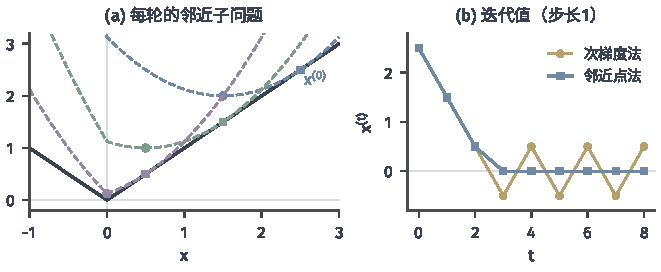
\includegraphics[width=112mm]{figures/03-optimization-evolution-and-signals/01-optimization/matplotlib/c4-prox-point/figure.pdf}
  \caption{邻近点法与次梯度法在$f(x)=|x|$上的比较（$\eta=1$，初值$2.5$）。(a) 黑线是$|x|$；三条虚线是以$x^{(t)}=2.5,1.5,0.5$为中心的子问题$|x|+(x-x^{(t)})^2/2$，方块标出当前点，圆点标出子问题最小点，也就是下一迭代点。(b) 迭代值随$t$的变化：邻近点法第三步到达$0$后停住，次梯度法在$0.5$与$-0.5$之间振荡。}
  \label{fig:opt-ns-prox-point}
\end{figure}

\paragraph{目标差与参数收敛}
下面在凸、最小点存在、子问题精确求解的条件下给出保证。

\begin{theorem}[邻近点法的收敛]
\label{thm:opt-ns-proximal-point}
设$f$适当、下半连续、凸，最小点集合非空，$\eta>0$固定，迭代~\eqref{eq:opt-ns-proximal-point}精确执行。则对任意最小点$\bm x^\star$，距离$\lVert\bm x^{(t)}-\bm x^\star\rVert_2$关于$t$不增，且
\[
 f(\bm x^{(T)})-f^\star\leq\frac{\lVert\bm x^{(0)}-\bm x^\star\rVert_2^2}{2\eta T}.
\]
进一步，整个序列$\bm x^{(t)}$收敛到某个最小点。
\end{theorem}

\begin{proof}
在定理~\ref{thm:opt-ns-prox-characterization}的条件(3)中取$r=f$、$\bm z=\bm x^{(t)}$、$\bm p=\bm x^{(t+1)}$、$\bm y=\bm x^\star$，并略去右端的非负项$\lVert\bm x^{(t+1)}-\bm x^{(t)}\rVert_2^2/(2\eta)$，得
\[
 f(\bm x^{(t+1)})-f^\star\leq\frac1{2\eta}\Bigl(\lVert\bm x^{(t)}-\bm x^\star\rVert_2^2-\lVert\bm x^{(t+1)}-\bm x^\star\rVert_2^2\Bigr).
\]
左端非负，所以距离不增。对$t=0,\dots,T-1$求和，右端相消为不超过$\lVert\bm x^{(0)}-\bm x^\star\rVert_2^2/(2\eta)$；由式~\eqref{eq:opt-ns-proximal-point-descent}，$f(\bm x^{(t)})$不增，左端之和不小于$T\bigl(f(\bm x^{(T)})-f^\star\bigr)$，得到目标差界。

对参数收敛：距离不增说明序列有界，因而有收敛子列$\bm x^{(t_k)}\to\bar{\bm x}$。目标差界说明$f(\bm x^{(t)})\to f^\star$，由下半连续性$f(\bar{\bm x})\leq\liminf_kf(\bm x^{(t_k)})=f^\star$，所以$\bar{\bm x}$是最小点。把距离不增用于$\bm x^\star=\bar{\bm x}$：$\lVert\bm x^{(t)}-\bar{\bm x}\rVert_2$不增，又有一个子列趋于零，故整个序列趋于$\bar{\bm x}$。
\end{proof}

最小点不唯一时，极限是哪一个最小点由初值决定，定理只保证收敛到其中某一个。

\paragraph{代价与不精确求解}
邻近点法没有步长上限，也不需要光滑性，代价转移到了子问题上：每一轮都要精确求解一个与原问题几乎同样困难的强凸问题。例如对最小二乘目标$f(\bm x)=\frac12\lVert\bm A\bm x-\bm b\rVert_2^2$，每轮需要解线性方程组$(\bm A^\top\bm A+\bm I/\eta)\bm x=\bm A^\top\bm b+\bm x^{(t)}/\eta$，代价与直接求解原问题同阶。因此“不受光滑常数限制”不意味着总计算量更少。

实践中子问题只能近似求解。此时必须规定误差标准，例如要求实际输出与精确邻近点的距离不超过预先给定的$\epsilon^{(t)}$，并让这些误差足够快地减小；精确情形的证明不能直接搬用，需要把每轮误差加进上面的不等式重新累计。邻近点法真正的价值在于提供隐式更新的模板：下一节只把目标中简单的那一部分放进邻近子问题，其余部分用梯度近似，从而把每轮子问题变得便宜。

\section{光滑项与非光滑项的复合}
\label{sec:opt-ns-composite}

章首的$\ell_1$正则最小二乘有一个共同的结构：目标是一个光滑项与一个非光滑项之和，光滑项的梯度容易计算，非光滑项的邻近映射容易计算。本节研究这样的\term{复合目标}（composite objective）
\begin{equation}
 F(\bm x)=f(\bm x)+r(\bm x),
 \label{eq:opt-ns-composite}
\end{equation}
其中$f:\mathbb R^d\to\mathbb R$可微且梯度$L$-Lipschitz（第~\ref{chap:opt-smooth}章称为$L$光滑），$r$是适当、下半连续的凸函数，其邻近映射容易计算。对整个$F$用次梯度法，浪费了$f$的光滑性和$r$的简单结构；对整个$F$用邻近点法，子问题又太难。折中的办法是只近似$f$、完整保留$r$，并要求这样做仍能控制原目标$F$的进展。

\subsection{邻近梯度法}
\label{sec:opt-ns-proximal-gradient}

第~\ref{chap:opt-smooth}章的下降引理给出$L$光滑函数的二次上界：对所有$\bm x,\bm y$，
\begin{equation}
 f(\bm y)\leq f(\bm x)+\langle\nabla f(\bm x),\bm y-\bm x\rangle+\frac L2\lVert\bm y-\bm x\rVert_2^2 .
 \label{eq:opt-ns-descent-lemma}
\end{equation}
在那里，最小化右端得到梯度步$\bm x-\nabla f(\bm x)/L$。现在目标多了$r$。保留$r$不动，只把$f$换成它的二次上界，并把系数$L$换成$1/\eta$（$0<\eta\leq1/L$时这仍是上界），得到当前点$\bm x$处的模型
\[
 m_{\bm x}(\bm y)=f(\bm x)+\langle\nabla f(\bm x),\bm y-\bm x\rangle+\frac1{2\eta}\lVert\bm y-\bm x\rVert_2^2+r(\bm y).
\]

\paragraph{配方得到更新}
模型中关于$\bm y$的一次项和二次项可以配方：
\[
 \langle\nabla f(\bm x),\bm y-\bm x\rangle+\frac1{2\eta}\lVert\bm y-\bm x\rVert_2^2
 =\frac1{2\eta}\bigl\lVert\bm y-\bigl(\bm x-\eta\nabla f(\bm x)\bigr)\bigr\rVert_2^2-\frac\eta2\lVert\nabla f(\bm x)\rVert_2^2 .
\]
去掉与$\bm y$无关的项，最小化模型就是以梯度步的终点为中心求$r$的邻近映射。\term{邻近梯度法}（proximal gradient method）因此写成
\begin{equation}
 \bm x^{(t+1)}=\operatorname{prox}_{\eta r}\bigl(\bm x^{(t)}-\eta\nabla f(\bm x^{(t)})\bigr).
 \label{eq:opt-ns-proximal-gradient}
\end{equation}
一轮分两步：先对光滑项做一次显式梯度步，形成中心；再对非光滑项做一次隐式的邻近步。$r=0$时它退化为梯度下降；$f=0$时它就是邻近点法；$r=\iota_C$时邻近步是投影，得到第~\ref{chap:constrained-optimization}章的投影梯度法。

\begin{example}[二维Lasso的第一步]
\label{ex:opt-ns-lasso-step}
取$\bm A=\begin{pmatrix}1&1\\1&0\end{pmatrix}$、$\bm b=(1,2)^\top$、$\lambda=1$，目标$F(\bm x)=\frac12\lVert\bm A\bm x-\bm b\rVert_2^2+\lVert\bm x\rVert_1$。光滑部分的梯度为$\bm A^\top\bm A\bm x-\bm A^\top\bm b$，其中$\bm A^\top\bm A=\begin{pmatrix}2&1\\1&1\end{pmatrix}$、$\bm A^\top\bm b=(3,1)^\top$；最大特征值$L=(3+\sqrt5)/2\approx2.618$，取$\eta=1/4\leq1/L$。

从$\bm x^{(0)}=(-1,2)^\top$出发：梯度为$(-2+2-3,\ -1+2-1)^\top=(-3,0)^\top$，梯度步的中心是$(-1,2)^\top-\frac14(-3,0)^\top=(-0.25,2)^\top$；再以阈值$\eta\lambda=0.25$做软阈值，得$\bm x^{(1)}=(0,1.75)^\top$。第一个坐标被精确置零，目标值从$7.5$降到$4.03125$。

最优解可以由最优条件直接核验。猜测$x_2^\star=0$、$x_1^\star>0$：第一个坐标要求$2x_1-3+1=0$，得$x_1^\star=1$；第二个坐标要求$|[\bm A^\top(\bm b-\bm A\bm x^\star)]_2|=|1-x_1^\star|=0\leq1$，成立。所以$\bm x^\star=(1,0)^\top$，$F^\star=1.5$。只看光滑部分，最小点却是$(\bm A^\top\bm A)^{-1}\bm A^\top\bm b=(2,-1)^\top$。
\end{example}

图~\ref{fig:opt-ns-lasso-path}画出邻近梯度法在这个例子上的完整路径。紫色箭头是第一轮的梯度步，红色箭头是随后的软阈值。路径在第7步到达横轴，此后第二个坐标一直是精确的零，第一个坐标沿横轴逼近$1$。作为对照，只对光滑部分做梯度下降的黄色路径直奔$(2,-1)^\top$，其中两个坐标都不为零。$\ell_1$项把解拉到坐标轴上，而且是精确地落在轴上，这来自每一轮软阈值的零区间。

\begin{figure}[!htbp]
  \centering
  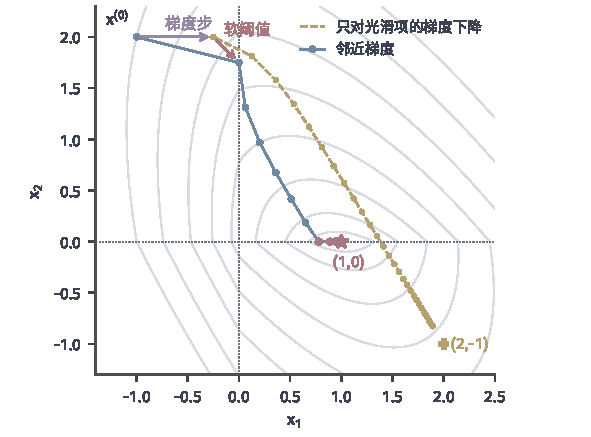
\includegraphics[width=100mm]{figures/03-optimization-evolution-and-signals/01-optimization/matplotlib/c4-lasso-path/figure.pdf}
  \caption{邻近梯度法在二维Lasso上的路径。灰色曲线是$F(\bm x)=\frac12\lVert\bm A\bm x-\bm b\rVert_2^2+\lVert\bm x\rVert_1$的等高线（$\bm A,\bm b$见例~\ref{ex:opt-ns-lasso-step}），红星是最小点$(1,0)$。蓝色折线是$\eta=1/4$的邻近梯度法，第一轮分解为紫色的梯度步和红色的软阈值；红色圆点标出第二个坐标恰为零的迭代点（从第7步起）。黄色虚线是只对光滑部分做梯度下降的路径，趋向光滑部分的最小点$(2,-1)$。}
  \label{fig:opt-ns-lasso-path}
\end{figure}

\paragraph{原目标的下降}
邻近梯度法近似了$f$，需要说明原目标$F$仍然受控。记$\bm x^+=\operatorname{prox}_{\eta r}(\bm x-\eta\nabla f(\bm x))$、$\bm d=\bm x^+-\bm x$。邻近最优条件（定理~\ref{thm:opt-ns-prox-characterization}的条件(2)）给出$-\bm d/\eta-\nabla f(\bm x)\in\partial r(\bm x^+)$；把这条次梯度的支撑不等式用于旧点$\bm x$，
\[
 r(\bm x)\geq r(\bm x^+)+\Bigl\langle-\frac{\bm d}\eta-\nabla f(\bm x),-\bm d\Bigr\rangle=r(\bm x^+)+\frac1\eta\lVert\bm d\rVert_2^2+\langle\nabla f(\bm x),\bm d\rangle .
\]
与下降引理$f(\bm x^+)\leq f(\bm x)+\langle\nabla f(\bm x),\bm d\rangle+\frac L2\lVert\bm d\rVert_2^2$相加，梯度项抵消，得
\begin{equation}
 F(\bm x^+)\leq F(\bm x)-\Bigl(\frac1\eta-\frac L2\Bigr)\lVert\bm x^+-\bm x\rVert_2^2 .
 \label{eq:opt-ns-proximal-gradient-descent}
\end{equation}
只要$0<\eta<2/L$，原目标就逐轮下降。这一推导没有用到$f$的凸性。

\paragraph{邻近梯度映射}
光滑优化用梯度范数衡量离驻点多远。复合目标的对应物是
\[
 \bm G_\eta(\bm x)=\frac{\bm x-\operatorname{prox}_{\eta r}\bigl(\bm x-\eta\nabla f(\bm x)\bigr)}\eta ,
\]
称为\term{邻近梯度映射}（proximal gradient mapping）。$r=0$时它就是$\nabla f(\bm x)$。它可以在每轮直接算出，并且有两条性质使它适合作停止量。

第一，$\bm G_\eta(\bm x)=\bm 0$当且仅当$\bm x$是邻近映射的不动点，由条件(2)这等价于$-\nabla f(\bm x)\in\partial r(\bm x)$，即$\bm 0\in\nabla f(\bm x)+\partial r(\bm x)$。称满足这一条件的点为复合目标的\term{复合临界点}（composite critical point），简称临界点。若$f$还是凸的，由于$f$在全空间有限，定理~\ref{thm:opt-ns-sum-rule}给出$\partial F=\nabla f+\partial r$，临界点就是全局最小点；$f$不凸时，它只是一阶必要条件。

第二，$\bm G_\eta(\bm x)$小，说明新点$\bm x^+$近似临界。由条件(2)，$\bm G_\eta(\bm x)-\nabla f(\bm x)\in\partial r(\bm x^+)$，所以向量$\nabla f(\bm x^+)-\nabla f(\bm x)+\bm G_\eta(\bm x)$属于$\nabla f(\bm x^+)+\partial r(\bm x^+)$，其范数不超过$L\lVert\bm x^+-\bm x\rVert_2+\lVert\bm G_\eta(\bm x)\rVert_2=(1+L\eta)\lVert\bm G_\eta(\bm x)\rVert_2$。

\paragraph{回溯与算法}
光滑常数$L$往往未知或偏保守。下降的证明只在一处用到$L$：新点满足二次上界。因此可以直接检验这个上界，不满足就缩小$\eta$重算。

\begin{algorithm}[带回溯的邻近梯度法]
  \label{alg:opt-ns-proximal-gradient}
  \begin{algorithmic}[1]
    \Require $f$的函数值与梯度，$r$的函数值与邻近映射；初值$\bm x^{(0)}\in\operatorname{dom}r$；初始步长$\eta>0$；缩小因子$\beta\in(0,1)$；容差$\varepsilon$
    \Ensure 近似临界点$\bm x$及其邻近梯度映射的范数
    \For{$t=0,1,2,\dots$}
      \State 计算$\nabla f(\bm x^{(t)})$
      \Loop
        \State $\bm x^+\gets\operatorname{prox}_{\eta r}\bigl(\bm x^{(t)}-\eta\nabla f(\bm x^{(t)})\bigr)$
        \If{$f(\bm x^+)\leq f(\bm x^{(t)})+\langle\nabla f(\bm x^{(t)}),\bm x^+-\bm x^{(t)}\rangle+\frac1{2\eta}\lVert\bm x^+-\bm x^{(t)}\rVert_2^2$}
          \State 跳出内层循环
        \EndIf
        \State $\eta\gets\beta\eta$
      \EndLoop
      \State $\bm x^{(t+1)}\gets\bm x^+$
      \If{$\lVert\bm x^{(t)}-\bm x^{(t+1)}\rVert_2/\eta\leq\varepsilon$}
        \State \Return $\bm x^{(t+1)}$
      \EndIf
    \EndFor
  \end{algorithmic}
\end{algorithm}

在算法~\ref{alg:opt-ns-proximal-gradient}中，检验条件一旦满足，上面的下降推导就可以把$L/2$换成$1/(2\eta)$，得到$F(\bm x^{(t+1)})\leq F(\bm x^{(t)})-\frac1{2\eta}\lVert\bm x^{(t+1)}-\bm x^{(t)}\rVert_2^2$。由下降引理，$\eta\leq1/L$时检验必然通过，所以步长不会缩小到$\beta/L$以下，内层循环有限次结束。每轮代价是一次梯度、若干次函数值与邻近映射；每次缩小步长都要重新计算邻近映射，因为中心变了。

\paragraph{固定预条件}
若用第~\ref{chap:opt-smooth}章的固定正定矩阵$\bm P$对梯度预条件，中心变成$\bm x-\eta\bm P\nabla f(\bm x)$，邻近步中的距离也必须换成相应的加权距离：
\[
 \bm x^+=\argmin_{\bm y}\Bigl\{r(\bm y)+\frac1{2\eta}\bigl(\bm y-\bm x+\eta\bm P\nabla f(\bm x)\bigr)^\top\bm P^{-1}\bigl(\bm y-\bm x+\eta\bm P\nabla f(\bm x)\bigr)\Bigr\}.
\]
这正是把模型中的$\frac1{2\eta}\lVert\bm y-\bm x\rVert_2^2$换成$\frac1{2\eta}(\bm y-\bm x)^\top\bm P^{-1}(\bm y-\bm x)$后配方的结果，相应的上界条件也要用这个加权距离检验。对角$\bm P=\operatorname{diag}(p_j)$配合$\ell_1$正则时，子问题仍然逐坐标分离，第$j$个坐标的阈值变为$\eta p_j\lambda$；一般的非对角$\bm P$会使子问题失去逐坐标的闭式解。只换中心而不换距离，所得更新的不动点一般不是原问题的临界点。

\paragraph{收敛保证}
下面在固定步长$0<\eta\leq1/L$下，分别对一般光滑项和凸光滑项给出保证。

\begin{theorem}[邻近梯度法的保证]
\label{thm:opt-ns-proximal-gradient}
设$F=f+r$如式~\eqref{eq:opt-ns-composite}，$0<\eta\leq1/L$固定，迭代~\eqref{eq:opt-ns-proximal-gradient}精确执行。
\begin{enumerate}
  \item 若$F$有下界$F_{\inf}>-\infty$，则$\displaystyle\min_{0\leq t<T}\lVert\bm G_\eta(\bm x^{(t)})\rVert_2^2\leq\frac{2\bigl(F(\bm x^{(0)})-F_{\inf}\bigr)}{\eta T}$。
  \item 若$f$还是凸的且最小点$\bm x^\star$存在，则$\displaystyle F(\bm x^{(T)})-F^\star\leq\frac{\lVert\bm x^{(0)}-\bm x^\star\rVert_2^2}{2\eta T}$。
\end{enumerate}
\end{theorem}

\begin{proof}
(1) $\eta\leq1/L$时$\frac1\eta-\frac L2\geq\frac1{2\eta}$，式~\eqref{eq:opt-ns-proximal-gradient-descent}化为$F(\bm x^{(t+1)})\leq F(\bm x^{(t)})-\frac\eta2\lVert\bm G_\eta(\bm x^{(t)})\rVert_2^2$。对$t=0,\dots,T-1$求和，左右相消后得$\frac\eta2\sum_t\lVert\bm G_\eta(\bm x^{(t)})\rVert_2^2\leq F(\bm x^{(0)})-F_{\inf}$，最小项不超过平均值。

(2) 先证一个三点不等式：对任意$\bm y$，记$\bm x^+$为$\bm x$的一步更新，
\begin{equation}
 F(\bm x^+)\leq F(\bm y)+\frac1{2\eta}\Bigl(\lVert\bm x-\bm y\rVert_2^2-\lVert\bm x^+-\bm y\rVert_2^2\Bigr).
 \label{eq:opt-ns-three-point}
\end{equation}
由下降引理与$\eta\leq1/L$，$f(\bm x^+)\leq f(\bm x)+\langle\nabla f(\bm x),\bm x^+-\bm x\rangle+\frac1{2\eta}\lVert\bm x^+-\bm x\rVert_2^2$；由$f$凸，$f(\bm x)\leq f(\bm y)-\langle\nabla f(\bm x),\bm y-\bm x\rangle$；由条件(2)给出的次梯度$\frac1\eta(\bm x-\bm x^+)-\nabla f(\bm x)\in\partial r(\bm x^+)$，$r(\bm x^+)\leq r(\bm y)+\langle\frac1\eta(\bm x-\bm x^+)-\nabla f(\bm x),\bm x^+-\bm y\rangle$。三式相加，含$\nabla f(\bm x)$的项全部抵消，得
\[
 F(\bm x^+)\leq F(\bm y)+\frac1\eta\langle\bm x-\bm x^+,\bm x^+-\bm y\rangle+\frac1{2\eta}\lVert\bm x^+-\bm x\rVert_2^2 .
\]
再用恒等式$2\langle\bm x-\bm x^+,\bm x^+-\bm y\rangle=\lVert\bm x-\bm y\rVert_2^2-\lVert\bm x^+-\bm y\rVert_2^2-\lVert\bm x-\bm x^+\rVert_2^2$，即得式~\eqref{eq:opt-ns-three-point}。取$\bm y=\bm x^\star$、$\bm x=\bm x^{(t)}$，对$t=0,\dots,T-1$求和，右端相消；由(1)中的单调性，$F(\bm x^{(T)})$不超过各轮目标值的平均，得结论。
\end{proof}

两条结论分别报告不同的对象。没有凸性时，只能保证某一轮的邻近梯度映射小，也就是找到一个近似临界点；这里的$O(1/T)$是平方残差的速率，残差本身是$O(1/\sqrt T)$，并且不说明临界点是否全局最优。$f$凸时，最后一个迭代点的目标差是$O(1/T)$，与第~\ref{chap:opt-smooth}章梯度下降在凸光滑目标上的速率相同：非光滑项$r$没有拖慢速率，代价是每轮多一次邻近映射。还要注意，每轮子问题的解$\bm x^{(t+1)}$只是当前模型的最小点，它与原问题最小点之间的差距，正是上面两条结论要控制的量，不能把“子问题已精确求解”误读为“原问题已解好”。

\subsection{加速邻近梯度法}
\label{sec:opt-ns-fista}

第~\ref{chap:opt-smooth}章的Nesterov加速梯度法在凸光滑目标上把$O(1/T)$提高到$O(1/T^2)$。它的做法是先沿上一步的位移外推，再在外推点求梯度。邻近梯度法可以用同样的方式加速，只需把梯度步换成邻近梯度步。

\paragraph{外推点与更新}
加速版本维护两个序列：记录点$\bm x^{(t)}$，以及只用于求梯度的外推点$\bm y^{(t)}$。每一轮在外推点上做一次邻近梯度步，得到新的记录点，再用新旧记录点的差外推出下一个求值点。外推系数由一个固定的数列确定。

\begin{algorithm}[加速邻近梯度法（FISTA）]
  \label{alg:opt-ns-fista}
  \begin{algorithmic}[1]
    \Require $f$的梯度，$r$的邻近映射；初值$\bm x^{(0)}$；步长$0<\eta\leq1/L$；迭代次数$T$
    \Ensure 记录点$\bm x^{(T)}$
    \State $\bm y^{(0)}\gets\bm x^{(0)}$，$\theta_0\gets1$
    \For{$t=0,1,\dots,T-1$}
      \State $\bm x^{(t+1)}\gets\operatorname{prox}_{\eta r}\bigl(\bm y^{(t)}-\eta\nabla f(\bm y^{(t)})\bigr)$ \Comment{在外推点求梯度}
      \State $\theta_{t+1}\gets\bigl(1+\sqrt{1+4\theta_t^2}\bigr)/2$
      \State $\beta^{(t)}\gets(\theta_t-1)/\theta_{t+1}$
      \State $\bm y^{(t+1)}\gets\bm x^{(t+1)}+\beta^{(t)}\bigl(\bm x^{(t+1)}-\bm x^{(t)}\bigr)$ \Comment{沿位移外推}
    \EndFor
  \end{algorithmic}
\end{algorithm}

算法~\ref{alg:opt-ns-fista}称为\term{加速邻近梯度法}（accelerated proximal gradient method），常用名FISTA\sidecite{beck2009fista}。它每轮的代价与邻近梯度法相同：一次梯度、一次邻近映射，外加两个向量的线性组合。系数$\beta^{(0)}=0$，此后依次约为$0.28,\ 0.43,\ 0.53,\dots$，逐渐趋于$1$。在例~\ref{ex:opt-ns-lasso-step}中，第一轮两种方法完全相同；从第二轮起外推开始起作用，前五轮的目标值分别为$4.03,\ 3.32,\ 2.67,\ 2.06,\ 1.56$，而邻近梯度法为$4.03,\ 3.32,\ 2.80,\ 2.38,\ 2.04$；到第10轮，两者的第一个坐标分别约为$0.997$和$0.972$（最优值为$1$）。

\begin{theorem}[加速邻近梯度法的目标差]
\label{thm:opt-ns-fista}
设$F=f+r$如式~\eqref{eq:opt-ns-composite}，$f$凸，最小点$\bm x^\star$存在，$0<\eta\leq1/L$，邻近映射精确计算。则算法~\ref{alg:opt-ns-fista}的记录点满足
\[
 F(\bm x^{(T)})-F^\star\leq\frac{2\lVert\bm x^{(0)}-\bm x^\star\rVert_2^2}{\eta(T+1)^2}.
\]
\end{theorem}

证明沿用第~\ref{chap:opt-smooth}章加速梯度法的势函数论证：把三点不等式~\eqref{eq:opt-ns-three-point}分别用于$\bm y=\bm x^{(t)}$和$\bm y=\bm x^\star$，按$\theta_t$加权组合，验证一个由目标差与到最小点距离组成的势函数逐轮不增；数列满足$\theta_{t+1}^2-\theta_{t+1}=\theta_t^2$及$\theta_t\geq(t+2)/2$，由此得到$(T+1)^2$的分母。完整推导见\sidecite[第4节]{beck2009fista}。与邻近梯度法相比，三点不等式是唯一用到$r$的地方；只要邻近步精确，非光滑项不影响加速论证。

\paragraph{加速不承诺单调}
定理只控制目标差的上界，不保证$F(\bm x^{(t)})$逐轮下降。外推点可能越过最小点，下一轮记录点的目标值随之上升。图~\ref{fig:opt-ns-ista-fista}在一个固定随机种子生成的Lasso问题上比较两种方法：$\bm A\in\mathbb R^{60\times100}$，奇数列与相邻偶数列高度相关，$\lambda$取$0.1\lVert\bm A^\top\bm b\rVert_\infty$，两种方法都用$\eta=1/L$。左图中，加速版本在第100轮的目标差约为$5\times10^{-6}$，而邻近梯度法约为$0.2$；右图放大后可见，加速版本的目标差呈波浪形起伏，600轮中有254轮目标值比上一轮更高。两条点线是定理~\ref{thm:opt-ns-proximal-gradient}与定理~\ref{thm:opt-ns-fista}给出的界，实际误差远在界以下：这些界是对所有满足条件的问题成立的最坏情形保证，而这个实例的局部曲率帮助两种方法都比界下降得快。

\begin{figure}[!htbp]
  \centering
  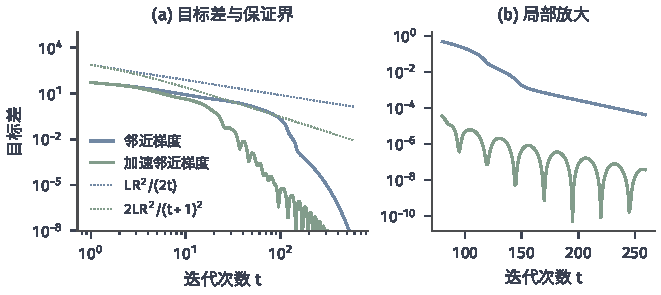
\includegraphics[width=112mm]{figures/03-optimization-evolution-and-signals/01-optimization/matplotlib/c4-ista-fista/figure.pdf}
  \caption{邻近梯度法与加速邻近梯度法在一个Lasso实例上的目标差（$n=60$，$d=100$，固定随机种子，参数见图源记录；$F^\star$由30000轮加速迭代估计）。(a) 双对数坐标下的$F(\bm x^{(t)})-F^\star$：蓝线为邻近梯度法，绿线为加速版本；点线为理论界$LR^2/(2t)$与$2LR^2/(t+1)^2$，$R=\lVert\bm x^{(0)}-\bm x^\star\rVert_2$。(b) 第80至260轮的放大（半对数坐标）：加速版本的目标差不单调，邻近梯度法单调下降。}
  \label{fig:opt-ns-ista-fista}
\end{figure}

\paragraph{实现时要配套的条件}
加速公式只是保证的一部分，以下几项改动都需要相应的条件。未知$L$时可以回溯，但检验必须在外推点$\bm y^{(t)}$处进行，即检验$f(\bm x^{(t+1)})\leq f(\bm y^{(t)})+\langle\nabla f(\bm y^{(t)}),\bm x^{(t+1)}-\bm y^{(t)}\rangle+\frac1{2\eta}\lVert\bm x^{(t+1)}-\bm y^{(t)}\rVert_2^2$，并且基本版本的分析要求步长只缩小、不放大。若需要单调的目标值，可以在目标上升时把外推系数重置为零，即“重启”；这在实践中常常有效，但重启后的速率需要另行分析，不能直接沿用定理~\ref{thm:opt-ns-fista}。邻近映射只能近似计算时，加速方法对误差更敏感：误差需要比非加速版本更快地趋于零，否则累积误差会抵消加速。$f$不凸时，上面的势函数论证不再成立，不能把$O(1/T^2)$的结论搬过去。

\section{光滑化}
\label{sec:opt-ns-smoothing}

邻近方法要求非光滑项有便宜的邻近映射。有限个仿射函数的最大值$\max_i\{\bm a_i^\top\bm x+b_i\}$就常常没有：它的邻近子问题是一个二次规划。另一条路是放弃精确保留尖点，用一个光滑函数整体替换原目标，再调用第~\ref{chap:opt-smooth}章的光滑方法。这样做引入了两种误差：替代函数与原函数之间的偏差，以及替代问题没有求准的误差。本节先构造最大值的光滑替代并计算偏差，再说明怎样在两种误差之间分配精度。

\subsection{最大值的光滑逼近}
\label{sec:opt-ns-smooth-max}

最大值函数的尖点出现在活跃分支切换的地方：在切换点一侧，梯度是一个分支的斜率；越过切换点，梯度立刻跳到另一个分支的斜率。要得到光滑函数，就要让这种切换在一个小范围内连续地完成。

\paragraph{对数和指数光滑化}
设$\varphi(\bm x)=\max_{1\leq i\leq m}\ell_i(\bm x)$，其中$\ell_i(\bm x)=\bm a_i^\top\bm x+b_i$。给定平滑参数$\nu>0$，令
\begin{equation}
 \varphi_\nu(\bm x)=\nu\log\sum_{i=1}^m\exp\Bigl(\frac{\ell_i(\bm x)}\nu\Bigr).
 \label{eq:opt-ns-lse}
\end{equation}
它称为对数和指数（log-sum-exp）\term{光滑化}（smoothing）。直观上，指数把较大的分支放大得远比较小的分支多，$\nu$越小，求和越由最大的那一项主导，对数再把它还原回原来的尺度。

偏差可以精确控制。记$M=\varphi(\bm x)$，把$e^{M/\nu}$提到求和号外：
\[
 \varphi_\nu(\bm x)=M+\nu\log\sum_{i=1}^m\exp\Bigl(\frac{\ell_i(\bm x)-M}\nu\Bigr).
\]
求和中每一项都在$(0,1]$内，并且取到最大值的那一项等于$1$，所以和介于$1$与$m$之间。于是对所有$\bm x$，
\begin{equation}
 \varphi(\bm x)\leq\varphi_\nu(\bm x)\leq\varphi(\bm x)+\nu\log m .
 \label{eq:opt-ns-lse-gap}
\end{equation}
偏差不依赖$\bm x$，也不依赖$\bm a_i,b_i$，只依赖分支数和$\nu$。

\paragraph{梯度与曲率}
对式~\eqref{eq:opt-ns-lse}求导，得
\[
 \nabla\varphi_\nu(\bm x)=\sum_{i=1}^mp_i(\bm x)\,\bm a_i,\qquad
 p_i(\bm x)=\frac{\exp(\ell_i(\bm x)/\nu)}{\sum_{k=1}^m\exp(\ell_k(\bm x)/\nu)} .
\]
权重$p_i$非负、和为$1$，是各分支的软化选择：活跃分支的权重最大，离活跃越远的分支权重以指数速度衰减。再求一次导数，Hessian为
\[
 \nabla^2\varphi_\nu(\bm x)=\frac1\nu\Bigl(\sum_ip_i\bm a_i\bm a_i^\top-\bar{\bm a}\bar{\bm a}^\top\Bigr),\qquad\bar{\bm a}=\sum_ip_i\bm a_i ,
\]
括号中是以$p_i$为权重的斜率协方差矩阵。它半正定，并且在半正定序下不超过$\sum_ip_i\bm a_i\bm a_i^\top$，后者又不超过$\max_i\lVert\bm a_i\rVert_2^2\,\bm I$。所以$\varphi_\nu$是凸函数，并且是$L_\nu$光滑的，$L_\nu=\max_i\lVert\bm a_i\rVert_2^2/\nu$。偏差界与光滑常数一起显示了平滑参数的两面：$\nu$越小，偏差$\nu\log m$越小，曲率上界$1/\nu$却越大，梯度方法可用的步长随之缩小。

\begin{example}[绝对值的两种光滑化]
\label{ex:opt-ns-abs-smoothing}
$|x|=\max\{x,-x\}$有$m=2$个分支。对数和指数光滑化为
\[
 \varphi_\nu(x)=\nu\log\bigl(e^{x/\nu}+e^{-x/\nu}\bigr),\qquad\varphi_\nu'(x)=\tanh(x/\nu),
\]
偏差在$x=0$处最大，等于$\nu\log2$。另一种常用的替代是Huber函数
\[
 h_\nu(x)=\begin{cases}x^2/(2\nu),&|x|\leq\nu,\\|x|-\nu/2,&|x|>\nu,\end{cases}\qquad h_\nu'(x)=\min\{\max\{x/\nu,-1\},1\},
\]
它把尖点附近长度为$2\nu$的一段换成抛物线，从下方逼近$|x|$，偏差$|x|-h_\nu(x)$在$[0,\nu/2]$内。两种替代的二阶导数都不超过$1/\nu$。图~\ref{fig:opt-ns-smooth-max}画出$\nu=0.5$时的情形。
\end{example}

\begin{figure}[!htbp]
  \centering
  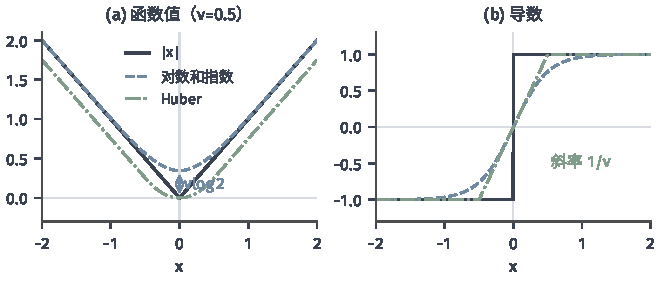
\includegraphics[width=112mm]{figures/03-optimization-evolution-and-signals/01-optimization/matplotlib/c4-smooth-max/figure.pdf}
  \caption{绝对值的两种光滑化（$\nu=0.5$）。(a) 黑线是$|x|$，蓝色虚线是对数和指数光滑化，从上方逼近，在原点的偏差为$\nu\log2\approx0.35$；绿色点划线是Huber函数，从下方逼近，偏差不超过$\nu/2$。(b) 对应的导数：$|x|$的导数在原点跳变，$\tanh(x/\nu)$与截断的直线$x/\nu$都连续地完成从$-1$到$1$的过渡，过渡区的斜率不超过$1/\nu$。}
  \label{fig:opt-ns-smooth-max}
\end{figure}

Huber函数最早作为稳健估计中的损失提出\sidecite{huber1964}，这里只用它的光滑性。图~\ref{fig:opt-ns-smooth-max}右图值得细看：原函数的导数在原点处从$-1$跳到$1$，两种替代都在宽度约为$\nu$的区间内连续地走完这段跳变。$\nu$减半，过渡区间变窄一半，过渡段的斜率加倍，这正是$L_\nu\propto1/\nu$的来源。

\paragraph{Huber函数是Moreau包络}
Huber函数并不是凭空设计的。对适当、下半连续的凸函数$f$，令
\[
 e_\nu f(\bm x)=\min_{\bm y}\Bigl\{f(\bm y)+\frac1{2\nu}\lVert\bm y-\bm x\rVert_2^2\Bigr\},
\]
称为$f$的\term{Moreau包络}（Moreau envelope）。它就是第~\ref{sec:opt-ns-prox}节邻近子问题的最优值，最小点是$\operatorname{prox}_{\nu f}(\bm x)$。对$f=|\cdot|$，代入软阈值：$|x|\leq\nu$时最小点是$0$，最优值为$x^2/(2\nu)$；$|x|>\nu$时最小点是$p=x-\nu\operatorname{sign}(x)$，$|p|=|x|-\nu$，距离项为$\nu^2/(2\nu)=\nu/2$，最优值为$|x|-\nu/2$。这正是$h_\nu$。一般地，Moreau包络是可微凸函数，梯度为$\bigl(\bm x-\operatorname{prox}_{\nu f}(\bm x)\bigr)/\nu$，且梯度是$1/\nu$-Lipschitz的\sidecite[第31节]{rockafellar1970convex}；对$|x|$可以直接验证：$\bigl(x-\operatorname{sign}(x)\max\{|x|-\nu,0\}\bigr)/\nu=h_\nu'(x)$。所以只要邻近映射可算，就能得到一个光滑替代；而对没有便宜邻近映射的最大值函数，对数和指数光滑化给出了另一条显式途径。

\paragraph{替代梯度不是原次梯度}
光滑化后，算法读取的是$\nabla\varphi_\nu(\bm x)=\sum_ip_i\bm a_i$。在远离切换点的地方，它接近活跃分支的斜率；在切换点附近，它是所有分支的软加权平均，这个向量一般不属于原函数在该点的次微分。例如$|x|$在$x=0.1$处的次微分是$\{1\}$，而$\nu=0.5$时$\tanh(0.2)\approx0.197$。因此光滑化方法不是“次梯度法换了一种选次梯度的方式”：它在每一轮求解的都是当前的光滑函数$\varphi_\nu$，收敛的对象也是$\varphi_\nu$的最小点，而不是原函数的最小点。两者之间的差距，要靠偏差界~\eqref{eq:opt-ns-lse-gap}来控制。

\subsection{偏差与求解精度}
\label{sec:opt-ns-smoothing-budget}

设原目标为$F=\phi+\varphi$，其中$\phi$是凸且$L_\phi$光滑的函数（可以为零），$\varphi$是上面的有限仿射最大值。用$F_\nu=\phi+\varphi_\nu$代替$F$，它是凸的且$(L_\phi+\max_i\lVert\bm a_i\rVert_2^2/\nu)$光滑。设$\widehat{\bm x}$是对$F_\nu$求解后返回的点，$F^\star$与$F_\nu^\star$分别是两个函数的最小值。

\paragraph{误差分解}
由式~\eqref{eq:opt-ns-lse-gap}，$F(\widehat{\bm x})\leq F_\nu(\widehat{\bm x})$；又对原问题任一最小点$\bm x^\star$，$F_\nu^\star\leq F_\nu(\bm x^\star)\leq F^\star+\nu\log m$。两式相减，
\begin{equation}
 F(\widehat{\bm x})-F^\star\leq\bigl(F_\nu(\widehat{\bm x})-F_\nu^\star\bigr)+\nu\log m .
 \label{eq:opt-ns-smoothing-split}
\end{equation}
右端第一项是替代问题的优化误差，可以靠增加迭代次数减小；第二项是替代本身的偏差，只取决于$\nu$。对固定的$\nu$，即使把替代问题完全求解，第二项仍然留在那里。

\paragraph{分配精度}
给定原目标的精度要求$\varepsilon$，自然的分配是两项各占一半：取$\nu=\varepsilon/(2\log m)$使偏差不超过$\varepsilon/2$，再把替代问题求解到优化误差不超过$\varepsilon/2$。设$\phi=0$、替代问题的最小点到初值的距离不超过$R$。第~\ref{chap:opt-smooth}章对凸$L$光滑目标给出：步长$1/L$的梯度下降$T$步后目标差不超过$LR^2/(2T)$，加速梯度法不超过$2LR^2/(T+1)^2$。代入$L_\nu=\max_i\lVert\bm a_i\rVert_2^2/\nu=2\log m\,\max_i\lVert\bm a_i\rVert_2^2/\varepsilon$，梯度下降需要约$L_\nu R^2/\varepsilon=O(\varepsilon^{-2})$次梯度计算，加速方法需要约$R\sqrt{4L_\nu/\varepsilon}=O(\varepsilon^{-1})$次。后者优于次梯度法的$O(\varepsilon^{-2})$次查询，但它依赖显式的最大值结构：每次梯度计算都要算出全部$m$个分支，任意的黑箱非光滑函数没有这种结构。

\begin{example}[固定平滑参数的平台]
\label{ex:opt-ns-smoothing-plateau}
在平面上取$m=5$个分支，斜率是单位圆上等分的五个方向$\bm a_i=(\cos\frac{2\pi(i-1)}5,\sin\frac{2\pi(i-1)}5)^\top$，截距$\bm b=(0,0.3,-0.2,0.5,0.1)^\top$。用线性规划求得原问题的最小值$F^\star\approx0.3065$。对$\nu=1,\ 0.1,\ 0.01$分别从$(3,2)^\top$出发，以步长$\nu$（即$1/L_\nu$）对$F_\nu$做梯度下降，并记录原目标的误差$F(\bm x^{(t)})-F^\star$。图~\ref{fig:opt-ns-smoothing-budget}显示：$\nu=1$时误差在10步内就降到约$0.09$并停住；$\nu=0.1$时约40步后停在约$0.026$；$\nu=0.01$时要约400步才开始快速下降，最终停在约$0.0026$。三个平台都在各自的偏差界$\nu\log5$（点线）以下。$\nu$越小，平台越低，但步长同样按$\nu$缩小，到达平台所需的步数也越多。
\end{example}

\begin{figure}[!htbp]
  \centering
  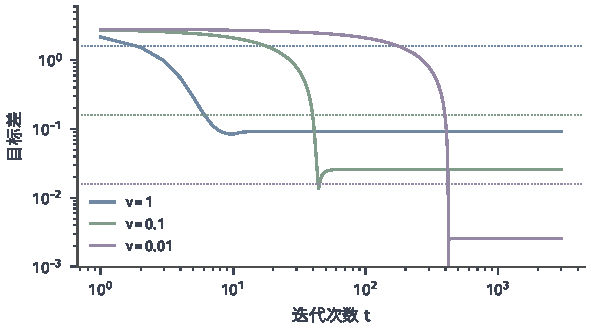
\includegraphics[width=100mm]{figures/03-optimization-evolution-and-signals/01-optimization/matplotlib/c4-smoothing-budget/figure.pdf}
  \caption{固定平滑参数的梯度下降在原目标上的误差（例~\ref{ex:opt-ns-smoothing-plateau}，双对数坐标）。蓝、绿、紫三条曲线分别对应$\nu=1,0.1,0.01$，步长均为$\nu$；同色点线是偏差界$\nu\log5$。每条曲线最终停在由$\nu$决定的平台上；$\nu$越小，平台越低，到达平台所需的迭代越多。}
  \label{fig:opt-ns-smoothing-budget}
\end{figure}

\paragraph{改变平滑参数}
实践中常从较大的$\nu$开始，得到粗略解后再缩小$\nu$，用上一阶段的结果作初值。每次缩小$\nu$，光滑常数$L_\nu$随之增大，必须重新确定步长，不能沿用旧$\nu$下的步长；相应的停止精度也要按新的偏差重新分配，新增的梯度计算要计入总预算。

\paragraph{替代目标下降，原目标未必下降}
梯度方法保证的是$F_\nu$的下降，原目标$F$可以在某一轮上升。再看例~\ref{ex:opt-ns-three-pieces}的$f(x)=\max\{-x,x/2,2x-3\}$，取$\nu=1$，$L_\nu\leq\max_ia_i^2/\nu=4$，步长$1/4$。从原问题的最小点$x=0$出发：三个分支在$0$处的值是$0,0,-3$，权重正比于$1,1,e^{-3}$，替代梯度为
\[
 \varphi_\nu'(0)=\frac{-1+\frac12+2e^{-3}}{2+e^{-3}}\approx-0.195 ,
\]
一步后到达$x\approx0.049$。替代函数值从$\log(2+e^{-3})\approx0.718$降到约$0.709$，原目标却从最小值$0$升到约$0.024$。原因是$F_\nu$的最小点不在$0$：$x/2$分支的软权重把它向右拉开了一段。式~\eqref{eq:opt-ns-lse-gap}只保证上升不超过$\nu\log m$，不保证逐轮不升。因此光滑化方法应同时记录替代目标和原目标，按式~\eqref{eq:opt-ns-smoothing-split}判断最终输出，而不是要求每一轮原目标都改善；这与下一节的代理模型不同，那里每轮都要用原目标检验改善。

\section{逐轮代理模型}
\label{sec:opt-ns-surrogates}

光滑化在开始时一次性地把原目标换成另一个函数，此后只求解替代函数。另一种思路是保留原目标不变，在每一轮围绕当前点重新构造一个容易求解的模型，用模型的最小点作为下一个候选。邻近梯度法已经是这样做的：它每轮使用的二次上界就是一个模型。本节把这一思路推广到两类模型。第一类是处处位于原目标上方、并在当前点接触的上界模型，它直接保证原目标下降，即MM方法；第二类是由已查询的支撑直线拼成的下界模型，它只能预测下降，候选点要查询原目标后才决定是否接受，即束方法。两类模型承担的作用不同，接受规则和保证也不同。

\subsection{MM的构造与更新}
\label{sec:opt-ns-mm}

回到邻近梯度法。式~\eqref{eq:opt-ns-descent-lemma}说明，$0<\eta\leq1/L$时模型$m_{\bm x}(\bm y)$处处不低于$F(\bm y)$，并且$m_{\bm x}(\bm x)=F(\bm x)$。正是这两条性质，加上新点使模型不高于当前值，保证了原目标下降。把这三条要求单独提出来，就不必限于二次上界。

\begin{definition}[主化代理与MM更新]
\label{def:opt-ns-mm}
设$F:\mathbb R^d\to\mathbb R\cup\{+\infty\}$，$\bm x^{(t)}\in\operatorname{dom}F$。函数$Q(\cdot\mid\bm x^{(t)})$若满足
\[
 Q(\bm x\mid\bm x^{(t)})\geq F(\bm x)\ \ \text{对所有}\ \bm x,\qquad Q(\bm x^{(t)}\mid\bm x^{(t)})=F(\bm x^{(t)}),
\]
就称为$F$在$\bm x^{(t)}$处的主化代理（majorizer）。选取满足$Q(\bm x^{(t+1)}\mid\bm x^{(t)})\leq Q(\bm x^{(t)}\mid\bm x^{(t)})$的新点，通常取代理的最小点，这样的迭代称为\term{主化--最小化方法}（majorization--minimization，MM）。
\end{definition}

三项要求依次是全域上界、当前点接触和代理改善。它们连成一条不等式链：
\begin{equation}
 F(\bm x^{(t+1)})\leq Q(\bm x^{(t+1)}\mid\bm x^{(t)})\leq Q(\bm x^{(t)}\mid\bm x^{(t)})=F(\bm x^{(t)}),
 \label{eq:opt-ns-mm-chain}
\end{equation}
第一步用上界，第二步用代理改善，第三步用接触。MM保证原目标逐轮不增，而且不需要原目标可微或凸，只需要能构造合格的代理。

\paragraph{为什么切线不行}
图~\ref{fig:opt-ns-mm-surrogates}左图比较$F(x)=x^2/2$在$x=1$处的两条曲线。主化代理$Q(x\mid1)=(x-1/2)^2+1/4$与$F$同值同斜率，并且$Q-F=(x-1)^2/2\geq0$，所以处处在上方；它的最小点$x=1/2$处$F(1/2)=1/8<1/2$，原目标确实下降。同一点的切线$x-1/2$也与$F$同值同斜率，但凸函数的切线在图像下方，不等式链的第一步反了；而且切线没有最小点，沿它下降会走到无穷远。可见“当前点同值同斜率”远不足以构成代理，关键在于全域的上方关系。

\begin{figure}[!htbp]
  \centering
  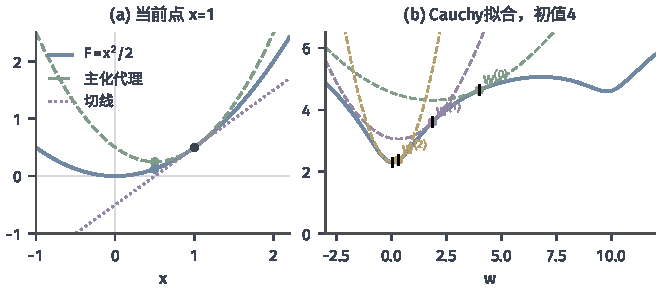
\includegraphics[width=112mm]{figures/03-optimization-evolution-and-signals/01-optimization/matplotlib/c4-mm-surrogates/figure.pdf}
  \caption{主化代理逐轮接触原目标。(a) 蓝线$F(x)=x^2/2$，绿色虚线是$x=1$处的主化代理$(x-1/2)^2+1/4$，紫色点线是同一点的切线$x-1/2$；代理在上方、切线在下方。代理的最小点$1/2$处，原目标从$1/2$降到$1/8$。(b) 蓝线是例~\ref{ex:opt-ns-cauchy-mm}的Cauchy拟合目标，三条虚线是从$w^{(0)}=4$开始前三轮的代理，每条都在当前点（圆点）接触目标、在别处位于上方，其最小点就是下一轮的当前点。}
  \label{fig:opt-ns-mm-surrogates}
\end{figure}

\paragraph{不精确求解代理}
代理子问题往往也要迭代求解，得到的只是近似最小点。记$Q^{\star,(t)}=\min_{\bm x}Q(\bm x\mid\bm x^{(t)})$，以及代理能提供的最大改善量$\Delta^{(t)}=Q(\bm x^{(t)}\mid\bm x^{(t)})-Q^{\star,(t)}\geq0$。若返回点满足$Q(\bm x^{(t+1)}\mid\bm x^{(t)})\leq Q^{\star,(t)}+\epsilon^{(t)}$，则由上界和接触，
\[
 F(\bm x^{(t+1)})\leq Q^{\star,(t)}+\epsilon^{(t)}=F(\bm x^{(t)})-\Delta^{(t)}+\epsilon^{(t)}.
\]
只有子问题误差$\epsilon^{(t)}$不超过可用改善量$\Delta^{(t)}$，本轮才保证不升。在左图的例子中，$Q^{\star}=1/4$，$\Delta=1/2-1/4=1/4$。若返回$x=3/4$，代理值$5/16$，误差$1/16\leq1/4$，原目标$F(3/4)=9/32<1/2$；若返回$x=5/4$，代理值$13/16$，误差$9/16>1/4$，原目标$F(5/4)=25/32$反而高于$1/2$。实现时最简单的检查是直接比较代理值：只要$Q(\bm x^{(t+1)}\mid\bm x^{(t)})\leq Q(\bm x^{(t)}\mid\bm x^{(t)})$，不等式链就成立。

\paragraph{局部代理}
有时上界只在当前点附近的区域$D^{(t)}$内成立，例如二次上界所用的曲率常数只在一个球内有效。这时不等式链的第一步只对$D^{(t)}$中的点成立，候选点必须限制在$D^{(t)}$内，代理子问题相应地带上这个约束。若不加限制地最小化代理，新点可能落在区域外，链就断了；局部有效的上界不能被无声地当作全局上界使用。

\paragraph{由凹性构造代理}
构造代理最常用的工具是凹函数在切线下方。设$\rho:[0,\infty)\to\mathbb R$可微、非减且凹，则$\rho(s)\leq\rho(s_0)+\rho'(s_0)(s-s_0)$对所有$s,s_0\geq0$成立。若目标形如$F(\bm x)=\frac12\sum_i\rho\bigl(r_i(\bm x)^2\bigr)$，其中$r_i$是残差，把每一项在当前残差平方$s_i^{(t)}=r_i(\bm x^{(t)})^2$处线性化，就得到
\begin{equation}
 Q(\bm x\mid\bm x^{(t)})=F(\bm x^{(t)})+\frac12\sum_ia_i^{(t)}\bigl(r_i(\bm x)^2-r_i(\bm x^{(t)})^2\bigr),\qquad a_i^{(t)}=\rho'(s_i^{(t)})\geq0 .
 \label{eq:opt-ns-irls-surrogate}
\end{equation}
它满足上界与接触两项要求，并且是残差的加权平方和：残差线性时，最小化代理就是一个加权最小二乘问题。每轮“由当前残差算权重、解加权最小二乘、更新残差”的方法称为\term{迭代重加权最小二乘}（iteratively reweighted least squares，IRLS）。拟合中的残差设计、权重退化与线性子问题的求解在第~\ref{chap:opt-function-fitting}章展开，这里只用一个标量例说明代理的构造。

\begin{example}[Cauchy损失的MM迭代]
\label{ex:opt-ns-cauchy-mm}
用一个常数$w$拟合数据$y=(0,0,10)$，目标为$F(w)=\frac12\sum_{i=1}^3\log\bigl(1+(w-y_i)^2\bigr)$，即$\rho(s)=\log(1+s)$，它凹且非减，$\rho'(s)=1/(1+s)$。由式~\eqref{eq:opt-ns-irls-surrogate}，代理的最小点是加权平均$w^{(t+1)}=\sum_ia_i^{(t)}y_i/\sum_ia_i^{(t)}$，权重$a_i^{(t)}=1/\bigl(1+(w^{(t)}-y_i)^2\bigr)$。

从$w^{(0)}=4$出发，权重为$(1/17,1/17,1/37)$，加权平均为$w^{(1)}=\frac{10/37}{2/17+1/37}\approx1.868$；下一轮权重约为$(0.223,0.223,0.015)$，得$w^{(2)}\approx0.324$；再下一轮得$w^{(3)}\approx0.058$。离群点$10$的权重随着它的残差增大而迅速变小，迭代趋向局部最小点$w\approx0.050$。从$w^{(0)}=0$出发，第一步权重为$(1,1,1/101)$，得$w^{(1)}=10/203\approx0.049$。图~\ref{fig:opt-ns-mm-surrogates}右图画出从$4$出发的前三个代理，每个都在当前点接触目标、在别处位于上方。

这个目标不是凸的，它在$w\approx9.789$处还有一个目标值更大的局部最小点（约$4.595$，而前者约$2.305$）。从$w^{(0)}=8$出发，MM迭代单调地收敛到$9.789$附近。不等式链只保证目标值不增，不保证到达全局最小点。
\end{example}

MM的适用范围不限于非光滑目标；光滑目标同样可以用二次上界或凹线性化构造代理。把它放在本章，是因为它与下面的束方法、上一节的光滑化一起，回答同一个问题：当原目标不便直接处理时，用什么样的辅助模型推进迭代。

\subsection{束方法}
\label{sec:opt-ns-bundle}

次梯度法每轮只用当前这一条支撑直线，用过就丢。对凸目标，每条查询到的支撑直线在全空间都是有效的下界，丢掉它们很浪费。\term{束方法}（bundle method）把查询过的支撑直线都保存下来，拼成原目标的一个分段线性下界模型，再加一个距离项防止候选点跑得太远。

\paragraph{割平面模型与稳定中心}
设$F:\mathbb R^d\to\mathbb R$是有限值凸函数，查询程序对每个点$\bm y$返回$F(\bm y)$和一条$\bm g\in\partial F(\bm y)$。设已经查询了点$\bm y_0,\dots,\bm y_k$，对应次梯度$\bm g_0,\dots,\bm g_k$。由支撑不等式，每条直线都在$F$下方，它们的最大值
\[
 m_k(\bm x)=\max_{0\leq j\leq k}\bigl\{F(\bm y_j)+\langle\bm g_j,\bm x-\bm y_j\rangle\bigr\}\leq F(\bm x)
\]
称为割平面模型，保存的这些直线合称为“束”。模型在每个查询点处与$F$相等，在其他地方是下界，越往查询点之外走，模型低估得越厉害。

只最小化$m_k$是危险的：它可能没有下界，例如只有一条支撑直线时；即使有最小点，也可能远离已知信息可靠的区域。因此束方法另外维护一个\term{稳定中心}（stability center）$\hat{\bm x}_k$，它是目前目标值最好的已接受点，并求解
\begin{equation}
 \bm y_{k+1}=\argmin_{\bm x}\Bigl\{m_k(\bm x)+\frac1{2\tau}\lVert\bm x-\hat{\bm x}_k\rVert_2^2\Bigr\}=\operatorname{prox}_{\tau m_k}(\hat{\bm x}_k),
 \label{eq:opt-ns-bundle-candidate}
\end{equation}
其中$\tau>0$。这是第~\ref{sec:opt-ns-prox}节的邻近子问题，只是把原目标换成了它的割平面模型：由定理~\ref{thm:opt-ns-prox-characterization}，解存在唯一。引入辅助变量$q$表示模型值，它可以写成二次规划：在约束$q\geq F(\bm y_j)+\langle\bm g_j,\bm x-\bm y_j\rangle$（$j=0,\dots,k$）下最小化$q+\lVert\bm x-\hat{\bm x}_k\rVert_2^2/(2\tau)$。

\paragraph{预测下降与接受检验}
模型在中心处是精确的（只要中心处的支撑直线在束中），所以$m_k(\hat{\bm x}_k)=F(\hat{\bm x}_k)$。模型预测，从中心移到候选点能使目标降低
\[
 \delta_k=F(\hat{\bm x}_k)-m_k(\bm y_{k+1}).
\]
由于$\bm y_{k+1}$是子问题的最小点，$m_k(\bm y_{k+1})+\lVert\bm y_{k+1}-\hat{\bm x}_k\rVert_2^2/(2\tau)\leq m_k(\hat{\bm x}_k)=F(\hat{\bm x}_k)$，所以$\delta_k\geq0$。但模型是下界，预测往往过于乐观，必须查询$F(\bm y_{k+1})$核验。给定$\beta\in(0,1)$，若实际下降至少是预测的$\beta$倍，
\[
 F(\hat{\bm x}_k)-F(\bm y_{k+1})\geq\beta\,\delta_k ,
\]
就接受候选点为新中心，称为\term{实质步}（serious step）；否则中心不动，称为\term{空步}（null step）。无论哪种情况，都把$\bm y_{k+1}$处的新支撑直线加入束。空步没有移动中心，却在模型低估最严重的地方补了一条割线，使下一次预测更准。

\begin{algorithm}[邻近束方法]
  \label{alg:opt-ns-bundle}
  \begin{algorithmic}[1]
    \Require 有限值凸函数$F$的函数值与次梯度程序；初值$\bm y_0$；参数$\tau>0$，$\beta\in(0,1)$；容差$\varepsilon$
    \Ensure 稳定中心$\hat{\bm x}$及证书$(e,\bm s)$
    \State 查询$F(\bm y_0)$与$\bm g_0$，束$\gets\{(\bm y_0,F(\bm y_0),\bm g_0)\}$，$\hat{\bm x}\gets\bm y_0$
    \For{$k=0,1,2,\dots$}
      \State 由式~\eqref{eq:opt-ns-bundle-candidate}求候选$\bm y_{k+1}$，计算$\delta_k=F(\hat{\bm x})-m_k(\bm y_{k+1})$
      \State $\bm s\gets(\hat{\bm x}-\bm y_{k+1})/\tau$，$e\gets\delta_k-\tau\lVert\bm s\rVert_2^2$
      \If{$\delta_k\leq\varepsilon$}
        \State \Return $\hat{\bm x}$，$(e,\bm s)$
      \EndIf
      \State 查询$F(\bm y_{k+1})$与$\bm g_{k+1}\in\partial F(\bm y_{k+1})$，把这条支撑直线加入束
      \If{$F(\hat{\bm x})-F(\bm y_{k+1})\geq\beta\delta_k$}
        \State $\hat{\bm x}\gets\bm y_{k+1}$ \Comment{实质步}
      \EndIf \Comment{否则为空步，中心不动}
    \EndFor
  \end{algorithmic}
\end{algorithm}

\begin{example}[一维束方法]
\label{ex:opt-ns-bundle-1d}
取$F(x)=|x-1|+x^2/4$，最小点$x^\star=1$，$F^\star=1/4$。查询程序在$x<1$时返回$x/2-1$，在$x\geq1$时返回$x/2+1$。取$\tau=1$、$\beta=1/2$，从$y_0=-2$出发。

第一轮：$F(-2)=4$，$g_0=-2$，模型$m_0(x)=4-2(x+2)=-2x$。子问题$-2x+(x+2)^2/2$的最小点是$y_1=0$，预测下降$\delta_0=4-0=4$；实际$F(0)=1$，下降$3\geq2$，实质步，中心移到$0$。注意$m_0$本身没有下界，正是距离项让子问题有解。

第二轮：加入$0$处的割线$1-x$，模型为$\max\{-2x,1-x\}$。子问题在$x>-1$时为$1-x+x^2/2$，最小点$y_2=1$，模型值$0$，预测下降$1$；实际$F(1)=1/4$，下降$3/4\geq1/2$，实质步，中心移到$1$。

第三轮：加入$1$处的割线$1/4+\tfrac32(x-1)$。在中心$1$附近，模型由$1-x$与这条新割线组成，两者交于$x=0.9$，模型值$0.1$；子问题的最小点就是$y_3=0.9$（模型在此的次微分$[-1,3/2]$加上距离项斜率$-0.1$含零）。预测下降$\delta_2=0.15$，实际$F(0.9)=0.3025$反而比中心高，空步。第四轮加入$0.9$处的割线后，候选点约为$0.9988$，预测下降只有约$0.0018$，实际目标约$0.2506$，仍是空步，但此时预测下降已经很小。图~\ref{fig:opt-ns-bundle}画出第二、三轮的模型。
\end{example}

\begin{figure}[!htbp]
  \centering
  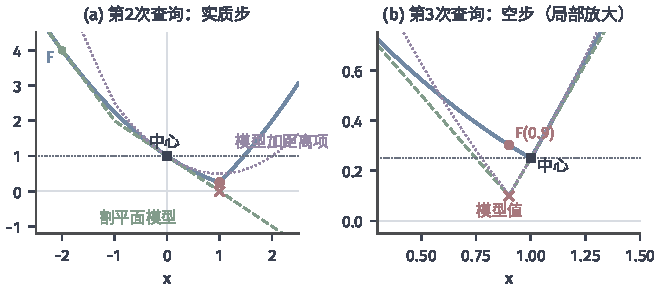
\includegraphics[width=112mm]{figures/03-optimization-evolution-and-signals/01-optimization/matplotlib/c4-bundle-model/figure.pdf}
  \caption{邻近束方法在$F(x)=|x-1|+x^2/4$上的两轮（例~\ref{ex:opt-ns-bundle-1d}，$\tau=1$）。蓝线是$F$，绿色虚线是由已查询点（绿点）的支撑直线拼成的割平面模型，紫色点线是模型加距离项，黑色方块是稳定中心，灰色点线标出中心处的目标值。红叉是候选点处的模型值，红点是候选点处的真实目标值。(a) 中心在$0$，候选点$1$的真实下降达到预测的一半以上，实质步。(b) 局部放大：中心在$1$，模型预测候选点$0.9$处的值为$0.1$，真实值却是$0.3025$，高于中心，空步。}
  \label{fig:opt-ns-bundle}
\end{figure}

\paragraph{可核验的停止标准}
预测下降不仅决定接受与否，还给出最优性证书。由于$\bm y_{k+1}=\operatorname{prox}_{\tau m_k}(\hat{\bm x}_k)$，邻近最优条件给出$\bm s_k=(\hat{\bm x}_k-\bm y_{k+1})/\tau\in\partial m_k(\bm y_{k+1})$。于是对所有$\bm x$，
\[
 F(\bm x)\geq m_k(\bm x)\geq m_k(\bm y_{k+1})+\langle\bm s_k,\bm x-\bm y_{k+1}\rangle
 =F(\hat{\bm x}_k)+\langle\bm s_k,\bm x-\hat{\bm x}_k\rangle-e_k ,
\]
其中$e_k=\delta_k-\tau\lVert\bm s_k\rVert_2^2$；最后一步用了$m_k(\bm y_{k+1})=F(\hat{\bm x}_k)-\delta_k$与$\langle\bm s_k,\hat{\bm x}_k-\bm y_{k+1}\rangle=\tau\lVert\bm s_k\rVert_2^2$。在上式中取$\bm x=\hat{\bm x}_k$，得$e_k\geq0$，因此$\tau\lVert\bm s_k\rVert_2^2\leq\delta_k$且$e_k\leq\delta_k$。上式说明$\bm s_k$是一条带误差$e_k$的近似次梯度；若已知某个最小点满足$\lVert\hat{\bm x}_k-\bm x^\star\rVert_2\leq R$，取$\bm x=\bm x^\star$即得
\[
 F(\hat{\bm x}_k)-F^\star\leq e_k+R\lVert\bm s_k\rVert_2\leq\delta_k+R\sqrt{\delta_k/\tau}.
\]
所以$\delta_k$小就同时控制了线性化误差和近似次梯度的大小。在例~\ref{ex:opt-ns-bundle-1d}第四轮，$\delta\approx0.0018$，$\lVert s\rVert=0.0012$，中心$1$正是最小点。

\paragraph{计算预算}
束方法的迭代次数不等于中心移动的次数。每一轮都要查询一次原目标（无论实质步还是空步）并求解一个二次规划，而二次规划的约束个数随束的增长而增长。报告计算量时要同时计入实质步、空步、原目标查询次数和每次子问题的求解代价；实践中还会定期合并或删去不再活跃的割线来控制束的大小，这需要额外的规则保证模型仍然有效。

\subsection{代理的保证与结果检验}
\label{sec:opt-ns-surrogate-guarantees}

上界模型、下界模型和固定的光滑替代都在用一个辅助函数推进迭代，但它们对原目标说了不同的话。本小节把三者放在同一个原目标下对照。

\paragraph{上模型与下模型不能互换}
MM的上界模型给出的是保证：代理值下降多少，原目标至少下降多少，由不等式链~\eqref{eq:opt-ns-mm-chain}直接得到，无需查询原目标。束方法的下界模型给出的只是预测：模型值下降，原目标可能上升，例~\ref{ex:opt-ns-bundle-1d}第三轮就是如此，所以每个候选点都必须查询原目标并通过接受检验。反过来，下界模型有上界模型没有的东西：它积累的割线给出了$F^\star$的下界和停止证书，而MM只能告诉我们目标值在下降，不能说明离最优还有多远。把下界模型当作上界使用会失去下降保证；把上界模型的最小值当作最优值的下界则是错误的。

光滑化又是第三种情形。它不在每轮重建模型，而是固定一个与原目标处处相差不超过$\nu\log m$的替代函数，然后只求解替代函数；它对原目标的控制完全来自偏差界~\eqref{eq:opt-ns-lse-gap}和误差分解~\eqref{eq:opt-ns-smoothing-split}，原目标在中间某些轮上升是允许的。表~\ref{tab:opt-ns-surrogates}汇总了三者的区别。

\begin{table}[!htbp]
  \centering
  \small
  \begin{tabularx}{\linewidth}{@{}l>{\raggedright\arraybackslash}X>{\raggedright\arraybackslash}X>{\raggedright\arraybackslash}X@{}}
    \toprule
     & MM & 束方法 & 光滑化 \\
    \midrule
    辅助函数 & 当前点处的主化代理，每轮重建 & 割平面下界模型，逐轮加割线 & 固定的光滑替代 \\
    与原目标的关系 & 处处在上方，当前点接触 & 处处在下方，查询点处相等 & 相差不超过$\nu\log m$ \\
    接受规则 & 代理值不增即可，无需查询原目标 & 实际下降不少于预测的$\beta$倍 & 无，按替代目标的方法运行 \\
    逐轮原目标 & 不增 & 中心处不增，候选点可升 & 可升，上升不超过$\nu\log m$ \\
    给出的保证 & 目标值单调；无最优间隙 & 停止证书$e_k+R\lVert\bm s_k\rVert_2$ & 原目标误差$\leq$优化误差$+\nu\log m$ \\
    \bottomrule
  \end{tabularx}
  \caption{三种辅助模型的对照。三者都作用于同一个原目标，但辅助函数与原目标的关系不同，因而接受规则和能报告的保证不同。}
  \label{tab:opt-ns-surrogates}
\end{table}

\paragraph{成本与返回对象}
三种方法的代价落在不同环节。MM的代价在构造代理和求解代理子问题，例如IRLS每轮解一个加权最小二乘；子问题只要求代理值不增，可以不精确求解。束方法的代价在原目标查询与越来越大的二次规划，空步消耗查询却不移动中心。光滑化的代价在梯度方法的迭代次数，它随$1/\nu$增长，改变$\nu$还要重新确定步长。返回时也要分清对象：MM返回最后一个迭代点；束方法返回稳定中心，而不是最后一个候选点，后者可能比中心差；光滑化返回替代问题的近似解，报告时应同时给出它的原目标值。

\paragraph{目标值收敛之后}
MM和束方法的中心都使原目标单调不增。若原目标有下界，单调有界的数列收敛，所以目标值序列收敛；但这只是目标值的收敛。迭代点是否收敛、极限是否为驻点、是否为全局最小点，都需要另外的条件。例~\ref{ex:opt-ns-cauchy-mm}从$8$出发收敛到一个非全局的局部最小点；对MM，证明极限点是驻点通常还要求代理在接触点处与目标的方向导数一致、代理关于当前点连续等条件。凸目标上束方法的收敛分析需要同时处理实质步与空步序列，篇幅较长，本章不展开，只使用上面可逐轮核验的停止证书：它不依赖收敛定理，每一轮都可以直接计算。

\section{本章小结}
\label{sec:opt-ns-summary}

章首问到，尖点处没有唯一斜率时还剩下什么信息。对凸目标，答案是全部全域支撑直线：它们组成次微分，在可微点退化为梯度，在尖点处是一个集合，例如$|x|$在原点的$[-1,1]$、有限最大值在切换点处活跃斜率的凸包。“零属于次微分”与全局最优等价，它是集合层面的判据，不要求算法读到的那一条次梯度为零。失去凸性后，Clarke广义梯度仍能记录局部斜率，但其中含零只是局部极小的必要条件。

只读一条支撑斜率时，负次梯度未必使目标下降，却总能使迭代点靠近最小点。次梯度法的保证因此落在历史最佳点或加权平均点上，目标差为$O(RG/\sqrt T)$，固定步长会留下平台。若非光滑项的邻近映射容易计算，就可以把它完整保留：邻近映射存在唯一、非扩张，其最优条件是在新点读取的次梯度；闭凸集的投影是它的特例，变分不等式和非扩张性都由此得到。邻近梯度法只对光滑项作二次上界近似，在凸情形保持$O(1/T)$的目标差，加速版本达到$O(1/T^2)$，但不再逐轮单调。

没有便宜的邻近映射时，有两条路。光滑化一次性地换成偏差可控的光滑函数，原目标误差分成优化误差与偏差两项，平滑参数同时决定偏差和曲率。代理模型则逐轮重建：MM的上界代理保证原目标单调不增，束方法的下界模型只预测下降，需要查询原目标决定实质步或空步，但它积累的割线给出了停止证书。表~\ref{tab:opt-ns-method-summary}按所需信息、保证与返回对象汇总这些方法。

\begin{table*}[!htbp]
  \centering
  \small
  \begin{tabularx}{\linewidth}{@{}l>{\raggedright\arraybackslash}X>{\raggedright\arraybackslash}X>{\raggedright\arraybackslash}X>{\raggedright\arraybackslash}X@{}}
    \toprule
    方法 & 每轮所需信息与代价 & 主要条件 & 保证的对象 & 返回点 \\
    \midrule
    次梯度法 & 一次函数值与一条次梯度 & 凸，次梯度有界，最小点存在 & 目标差$\leq(R^2+G^2\sum\eta_t^2)/(2\sum\eta_t)$ & 历史最佳点或加权平均点 \\
    邻近点法 & 整个目标的邻近子问题 & 适当、下半连续、凸，最小点存在 & 目标差$O(1/T)$，迭代点收敛 & 最后一点 \\
    邻近梯度法 & 一次梯度与一次邻近映射（回溯时多次） & $f$为$L$光滑，$r$凸且邻近映射易算 & 非凸：最小平方临界残差$O(1/T)$；凸：目标差$O(1/T)$ & 最后一点 \\
    加速邻近梯度法 & 同上，外加外推 & 同上且$f$凸 & 目标差$O(1/T^2)$，不保证单调 & 最后一个记录点 \\
    光滑化 & 替代函数的全部梯度 & 显式的有限最大值结构 & 原目标误差$\leq$优化误差$+\nu\log m$ & 替代问题的近似解 \\
    MM & 构造并近似求解代理 & 合格的全域上界代理 & 原目标单调不增 & 最后一点 \\
    束方法 & 一次查询与一个二次规划 & 有限值凸目标 & 停止证书$e_k+R\lVert\bm s_k\rVert_2$ & 稳定中心 \\
    \bottomrule
  \end{tabularx}
  \caption{本章方法的比较。各行的保证针对不同对象（目标差、临界残差或单调性），复杂度的计数单位也不同（一次查询、一次邻近映射或一个子问题），不能直接按阶数排序。}
  \label{tab:opt-ns-method-summary}
\end{table*}

比较这些方法时要分清三件事。第一，保证的对象：目标差、临界残差、目标单调与参数收敛各不相同，前一项成立不能推出后一项。第二，返回的点：次梯度法的界不针对最后一点，束方法应返回稳定中心而不是候选点。第三，计数单位：一次次梯度查询、一次邻近映射和一个完整子问题的代价相差可能很大，$O(1/\sqrt T)$与$O(1/T)$只有在单位可比时才能比较。

本章的各种保证都假定原问题有最小点；最小点是否存在、是否唯一，仍按第~\ref{chap:optimization}章的下半连续、紧下水平集与强凸条件判断，尖点本身既不帮助也不妨碍这些判断。例如$|x|+\frac\mu2x^2$非光滑却强凸，有唯一最小点；而邻近子问题总有唯一解，并不说明原问题如此。下一章处理约束：指示函数的邻近映射是投影，本章的投影性质在那里成为投影梯度法的基础，但约束的可行性、乘子与对偶证书需要新的工具。第~\ref{chap:opt-stochastic-block}章再处理只能读到带噪声梯度或次梯度的情形，那时本章的确定性误差界要换成期望意义下的界。

